\chapter{Diseño}

En el presente capítulo, se ofrece una descripción detallada de las clases que constituyen los diversos subsistemas, las bases de datos que almacenan la información crítica y los servidores que sustentan la operatividad del sistema. Se presentan, además, los diagramas de clases específicos para cada uno de estos subsistemas, proporcionando una visión clara de su estructura interna y las relaciones entre sus entidades. Adicionalmente, se incluyen diagramas de componentes que desglosan la arquitectura de las pantallas que conforman la aplicación móvil, ilustrando su organización y dependencias. Finalmente, se exploran los diagramas de secuencia, los cuales representan de manera exhaustiva las dinámicas trayectorias de interacción definidas por los casos de uso del sistema.

\section{Diagrama de la Estructura General del Sistema} 
La Figura \ref{fig:Diagrama de sistemas} ilustra la arquitectura general del proyecto propuesto, mostrando por separado cada uno de los diferentes sistemas que conforman este proyecto y el servicio en el que están alojados algunos de los sistemas. 
El presente diagrama muestra un sistema basado en microservicios, en el que se separa la lógica de la red neuronal de la parte del servidor. Por otro lado, dentro del servidor Java, apesar de tener toda la lógica dentro del mismo, existe la posibilidad de separar la lógica de la simulación del SAES, de la lógica del sistema móvil.

Como punto de partida está la base de datos, la cual está alojada en Railway. Esta abse de datos es la encargada de guardar todos los datos tanto de alumnos, docentes y el personal de seguridad, así como de otros datos académicos. Cabe recalcar que esta base de datos es una simulación de la base de datos de la página original del SAES, la cual se plantea compartir con el presente sistema móvil.

Posterior a esto, se tiene al servidor Java, el cual se encarga de procesar todas las solicitudes que haga el usuario dentro de la app móvil o del simulador del SAES. Esta parte del sistema se encuentra alojada en Azure. Este servidor se comunica tanto con el sistema web de la simulación del SAES, como con la app móvil, a través de solicitudes HTTPS.

A su vez, se encuentra el servidor de la red neuronal, alojado igualmente en Azure. Este servidor, como su nombre lo indica, se encarga únicamente de procesar todas las solicitudes para realizar el reconocimiento facial de los estudiantes dentro de la aplicación móvil. Sin embargo, para poder obtener los vectores de características de cada alumno y que se pueda hacer el reconocimiento facial de manera adecuada desde la app, se tiene la comunicación del sistema web con este mismo servidor. El sistema web cuenta con un módulo de registro de alumnos, en el cual se le toma un video de 5 segundos, para obtener diferentes fotos desde diferentes ángulos, y así, guardar el vector de características del alumno en el momento en el que se realizó su registro. De esta forma, al realizar el reconocimiento facial desde la aplicación móvil, tendrá un punto de partida para comparar con la foto que se le tome desde la aplicación móvil.

\begin{figure}[htbp!]
	\begin{center}
		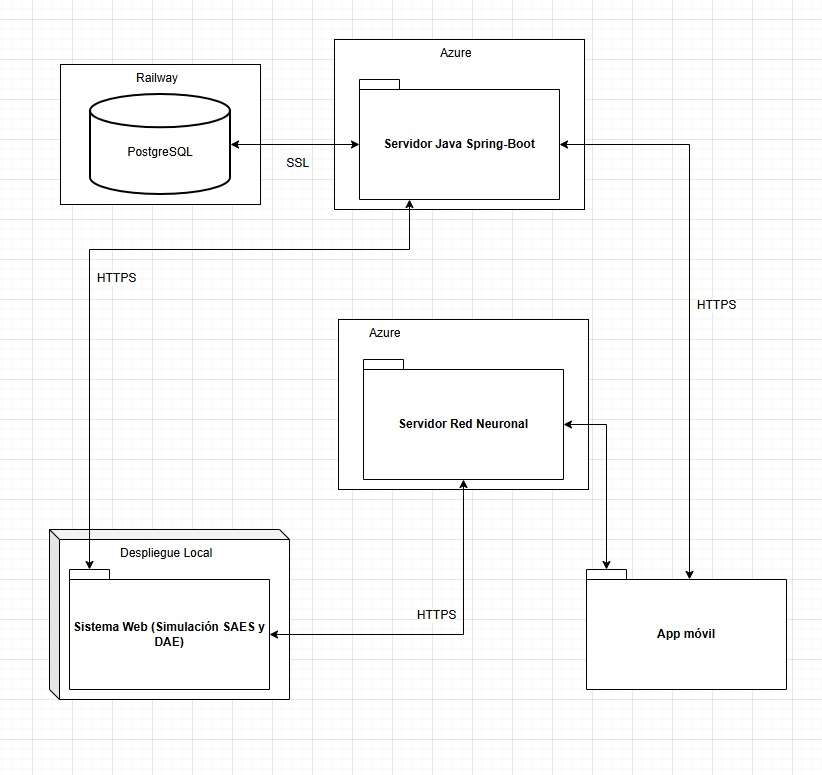
\includegraphics[width=0.9\textwidth]{images/DiagramaGeneralClases}
		\caption{Diagrama de la Estructura General del Sistema.}
		\label{fig:Diagrama de sistemas}
	\end{center}
\end{figure}

A continuación se entrara más en detalle en la estructura interna de los componentes del sistema del diagrama anterior.


\subsection{Estructura Interna del Servidor Spring Boot}
En la figura \ref{fig:DCG} se puede visualizar de manera general los componentes que conforman al servidor Java Spring Boot y el cómo se comunican.

Como punto de partida se tiene el paquete de los controladores (`com.example.PruebaCRUD.Controllers`). Estas clases son las encargadas de manejar las solicitudes HTTP que le llegan al servidor, así como de devolver una respuesta a dicha solicitud \cite{SpringController}. En otras palabras, estas clases son las encargadas de pasar la información entre la vista y el modelo. Para este caso en particular, estas clases se comunican con las clases de servicio, las cuales se encuentran en el paquete `com.example.PruebaCRUD.Services` y hacen uso de las clases que se encuentran en el paquete `com.example.PruebaCRUD.DTO`. 

Los DTO (Data Transfer Object), son clases que facilitan la transferencia de datos a través de la red o entre diferentes capas dentro del sistema \cite{DTO}. Como se puede ver dentro del diagrama, estos DTO son usados por la mayoría de las clases: las clases Controller, las cuales ya fueron descritas, así como las clases Service y Repository, de las cuales se explicarán a continuación.

Las clases de tipo Service son clases que se encargan de gestionar toda la lógica de negocio del sistema \cite{yadav-2024}. Funciona como intermediario entre los controladores y los repositorios.

Por otra parte, se encuentran los archivos de tipo Repository. Estos archivos son interfaces que permiten el acceso a la base de datos y el realizar operaciones CRUD \cite{diaz-2023}. Al extender de `JpaRepository`, estas interfaces heredan métodos para manipular entidades, eliminando la necesidad de implementar muchas de estas operaciones de manera manual.

Finalmente, se muestran a las clases de tipo Entity. Estas clases son parte de la capa de persistencia, y permiten mapear una clase Java, a una tabla de una base de datos \cite{pavan-2024}. De esta manera, las variables dentro de una clase, funcionarán como columnas dentro de una base de datos, haciendo que los datos que manda el usuario, se puedan guardar, actualizar, eliminar o consultar.

\newpage

\begin{figure}[htbp!]
	\begin{center}
		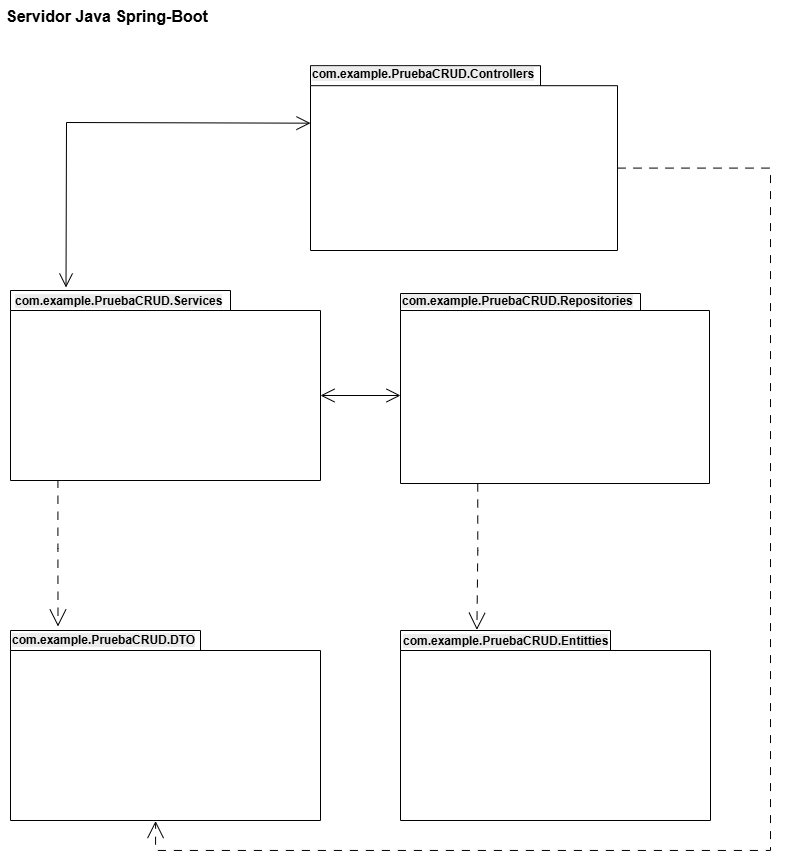
\includegraphics[width=0.8\textwidth]{Clases/DCG.png}
		\caption{Diagrama de la Estructura General del Servidor Java.}
		\label{fig:DCG}
	\end{center}
\end{figure}

A continuación, se presentan los diagramas de cada clase dentro de los paquetes explicados anteriormente.

\newpage
\subsubsection{Entidades}
A continuación, en las figuras \ref{fig:DCERed}, \ref{fig:DE1}, \ref{fig:DE2} y \ref{fig:DE3}, se mostrará más a detalle el contenido que tiene cada uno de los paquetes ilustrados anteriormente. Como primera parte, se muestran las clases que están dentro del paquete \\ `com.example.PruebaCRUD.Entities`. En este diagrama se muestran las relaciones internas entre las clases dentro del paquete ya mencionado.

\begin{figure}[htbp!]
	\begin{center}
		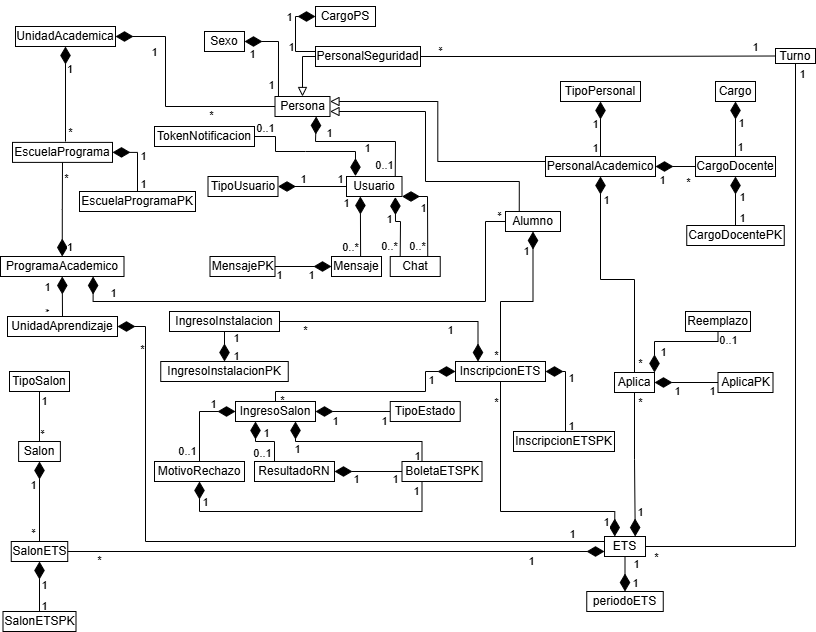
\includegraphics[width=0.8\textwidth]{Clases/DCE Reducido.png}
		\caption{Diagrama de clases general de las entidades del servidor.}
		\label{fig:DCERed}
	\end{center}
\end{figure}

 En este primer diagrama, las clases se muestran sin sus propiedades para una mejor visualización, sin embargo, en las imágenes posteriores se detalla más a profundidad las propiedades de cada una de estas clases.

\newpage

\begin{figure}[htbp!]
	\begin{center}
		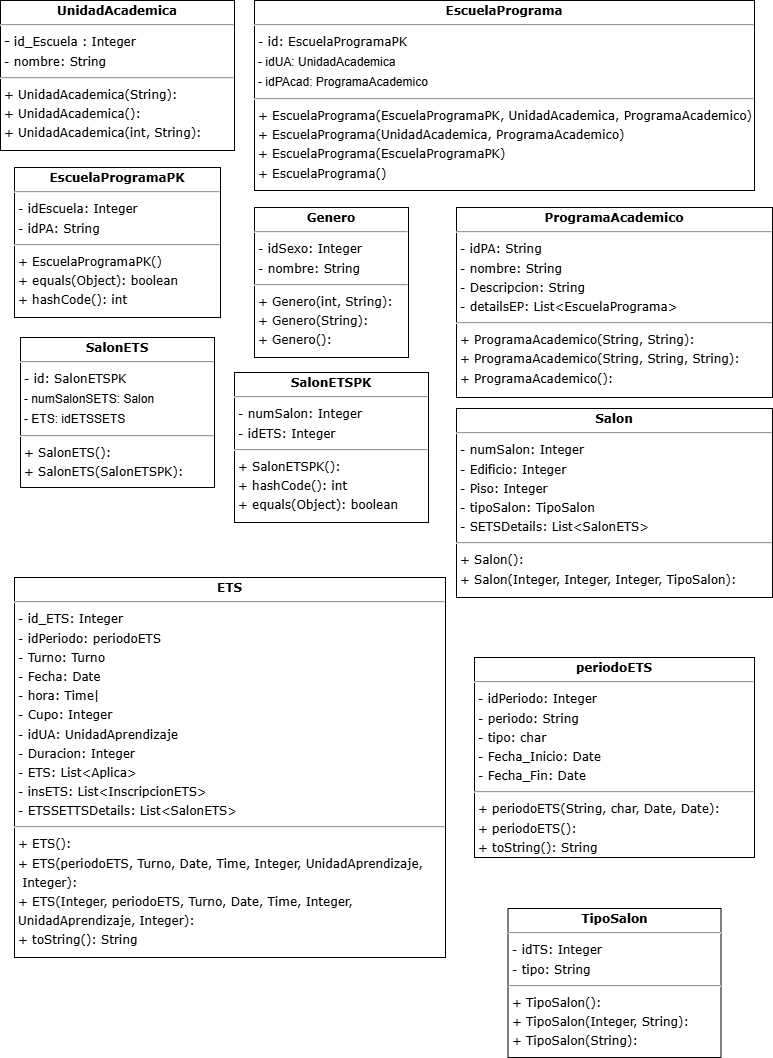
\includegraphics[width=0.8\textwidth]{Clases/EntidadesP1.png}
		\caption{Diagrama de clases de las entidades del servidor parte 1.}
		\label{fig:DE1}
	\end{center}
\end{figure}
\newpage

\begin{figure}[htbp!]
	\begin{center}
		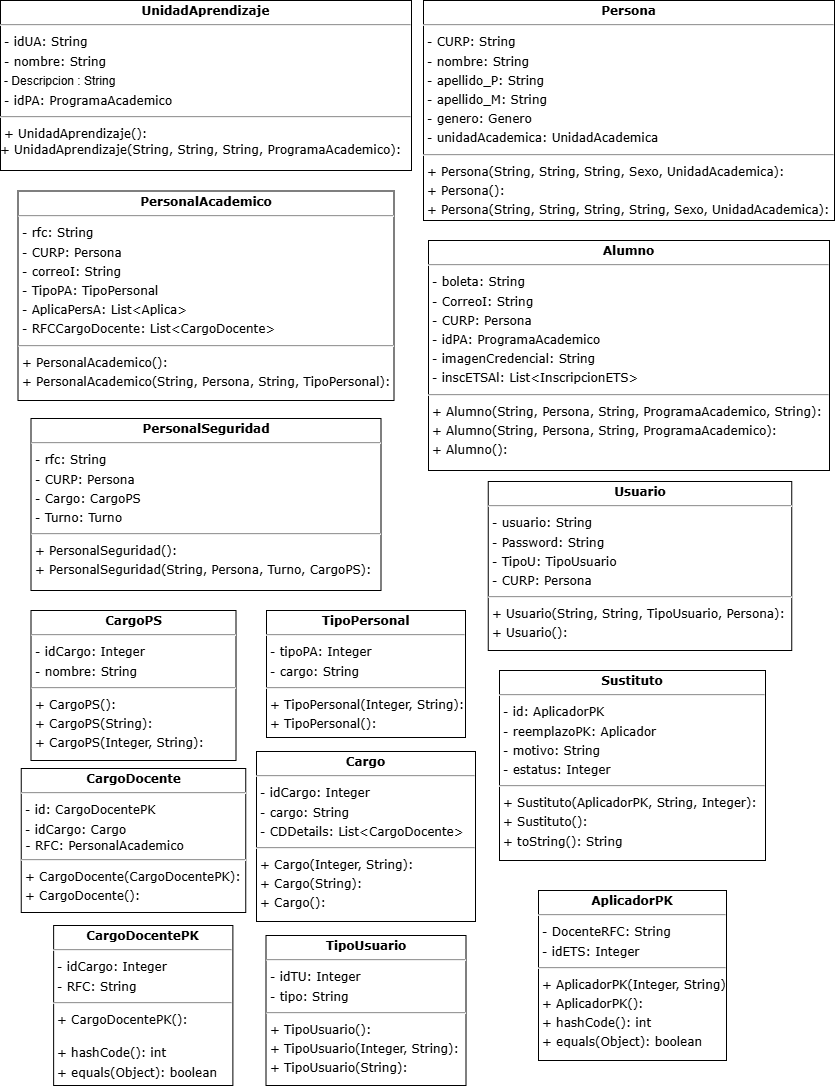
\includegraphics[width=0.8\textwidth]{Clases/EntidadesP2.png}
		\caption{Diagrama de clases de las entidades del servidor parte 2.}
		\label{fig:DE2}
	\end{center}
\end{figure}
\newpage

\begin{figure}[htbp!]
	\begin{center}
		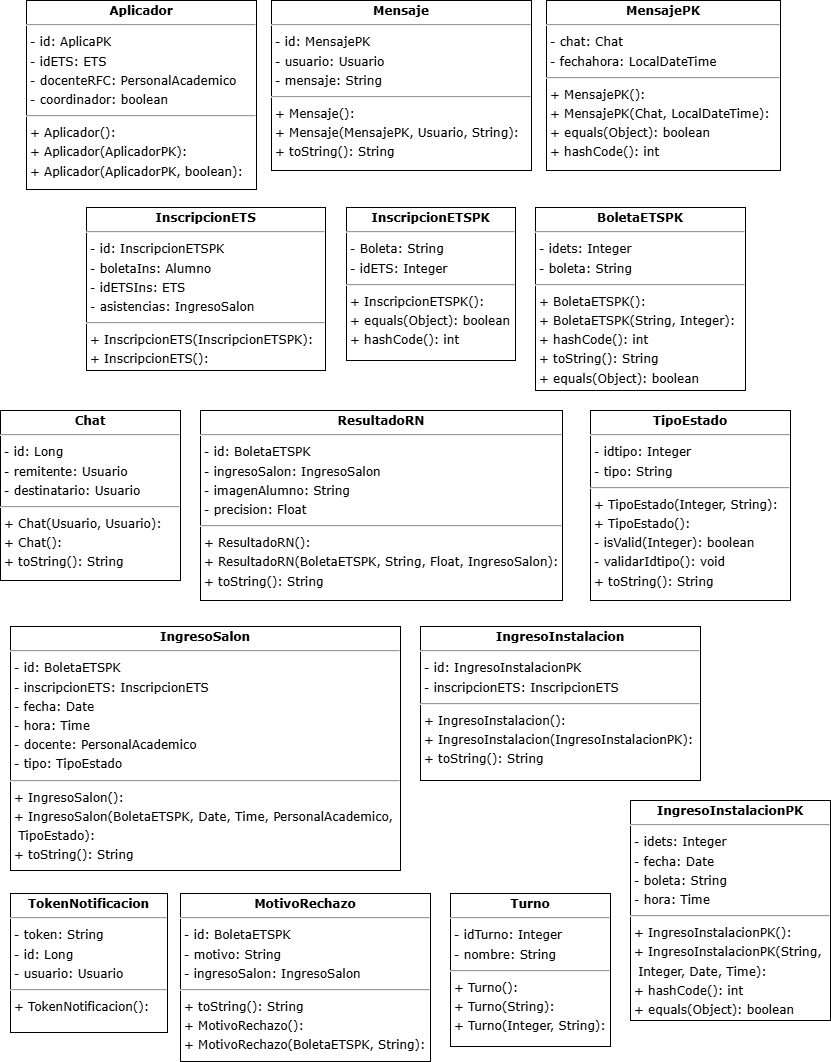
\includegraphics[width=0.8\textwidth]{Clases/EntidadesP3.png}
		\caption{Diagrama de clases de las entidades del servidor parte 3.}
		\label{fig:DE3}
	\end{center}
\end{figure}
\newpage
\subsubsection{Controladores}
En la figura \ref{fig:DC1}, \ref{fig:DC2}, \ref{fig:DC3}, \ref{fig:DC4} y \ref{fig:DC5}, se presentan los diagramas de las clases de los controladores junto con sus respectivas propiedades.

\begin{figure}[htbp!]
	\begin{center}
		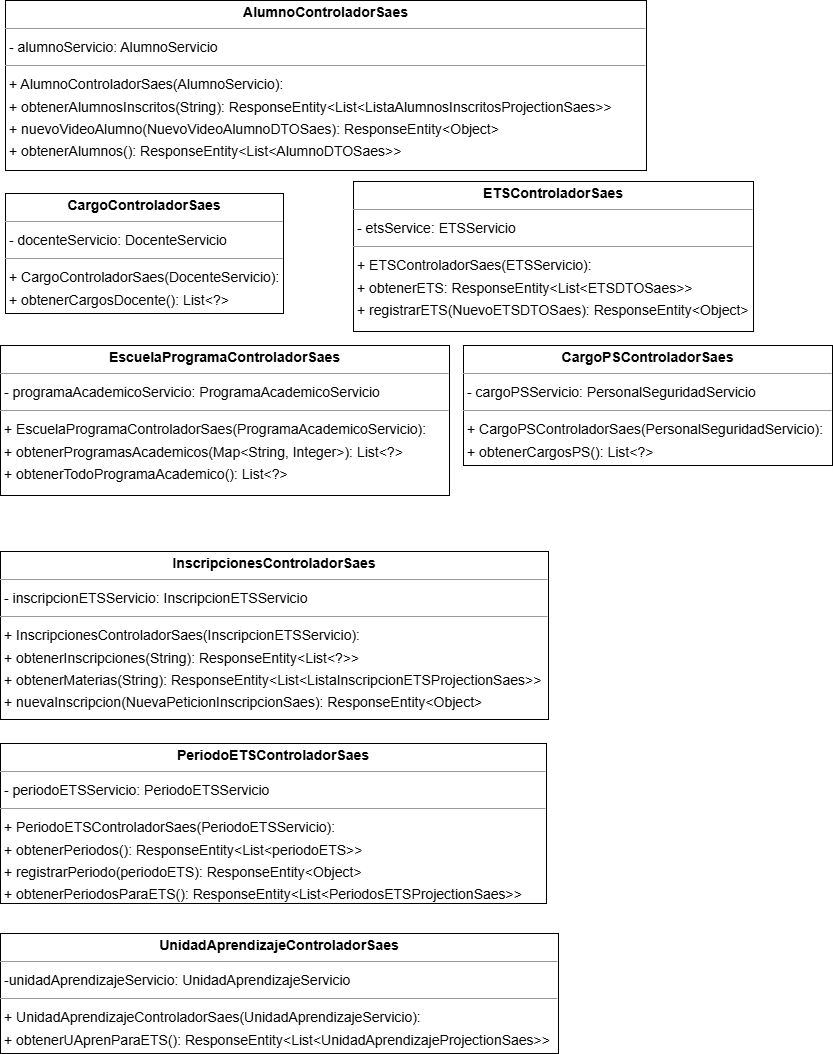
\includegraphics[width=0.7\textwidth]{Clases/Controlador1.png}
		\caption{Diagrama de clases de los controladores del servidor parte 1.}
		\label{fig:DC1}
	\end{center}
\end{figure}

\begin{figure}[htbp!]
	\begin{center}
		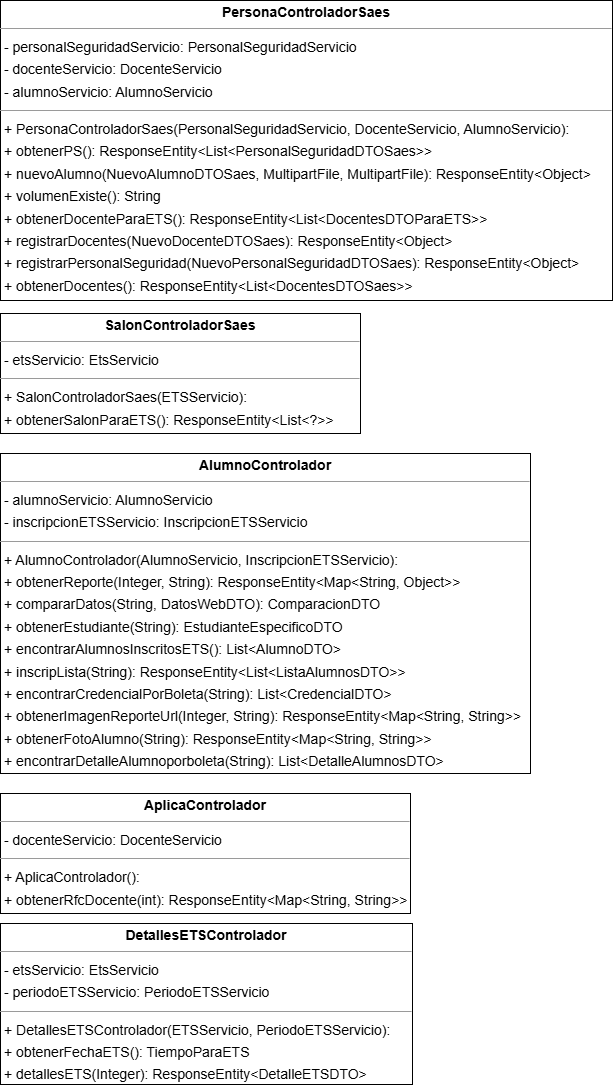
\includegraphics[width=0.65\textwidth]{Clases/Controlador2.png}
		\caption{Diagrama de clases de los controladores del servidor parte 2.}
		\label{fig:DC2}
	\end{center}
\end{figure}

\begin{figure}[htbp!]
	\begin{center}
		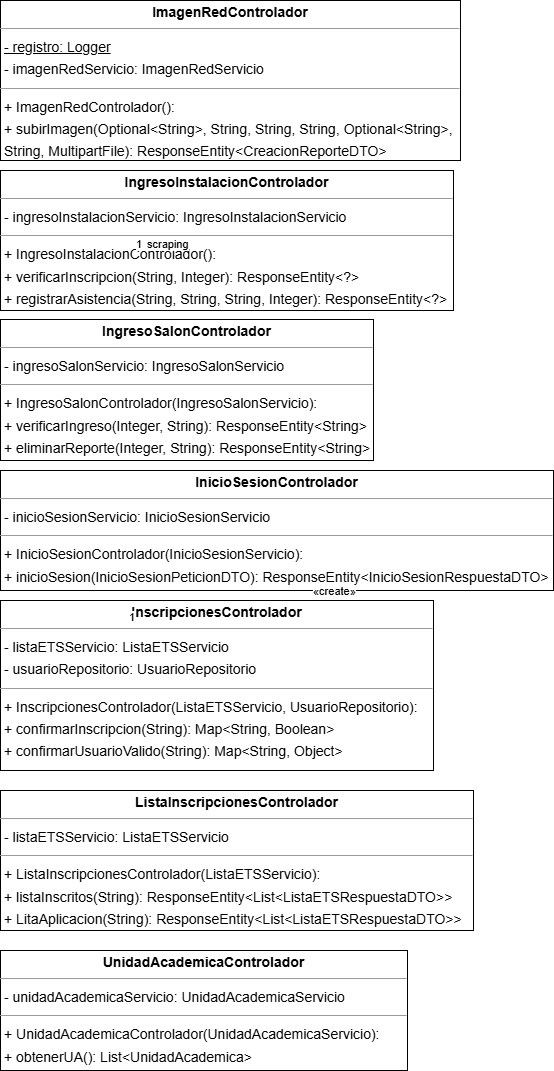
\includegraphics[width=0.6\textwidth]{Clases/Controlador3.png}
		\caption{Diagrama de clases de los controladores del servidor parte 3.}
		\label{fig:DC3}
	\end{center}
\end{figure}

\begin{figure}[htbp!]
	\begin{center}
		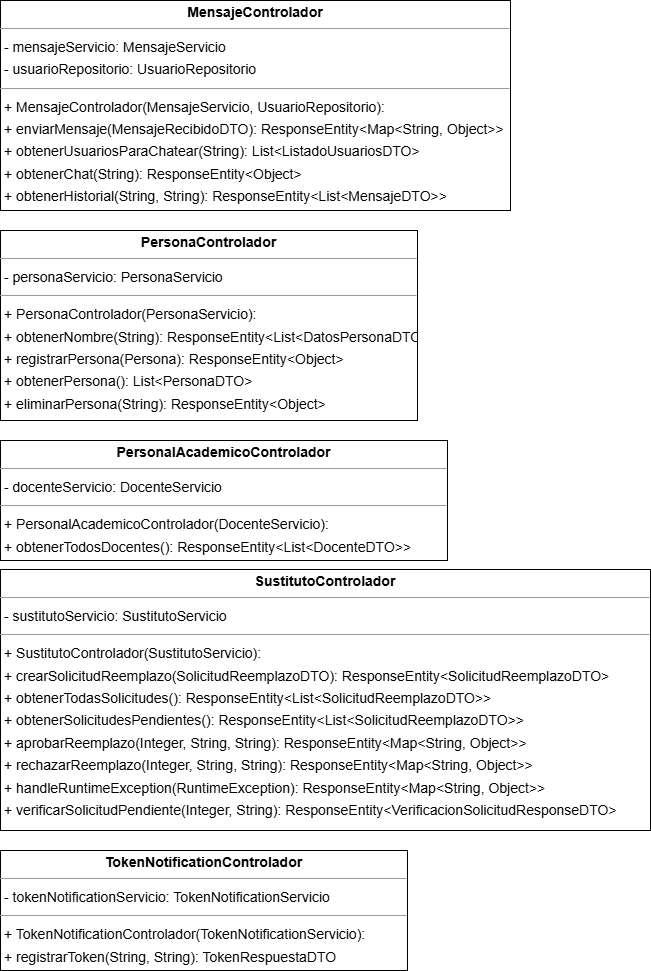
\includegraphics[width=0.75\textwidth]{Clases/Controlador4.png}
		\caption{Diagrama de clases de los controladores del servidor parte 4.}
		\label{fig:DC4}
	\end{center}
\end{figure}

\begin{figure}[htbp!]
	\begin{center}
		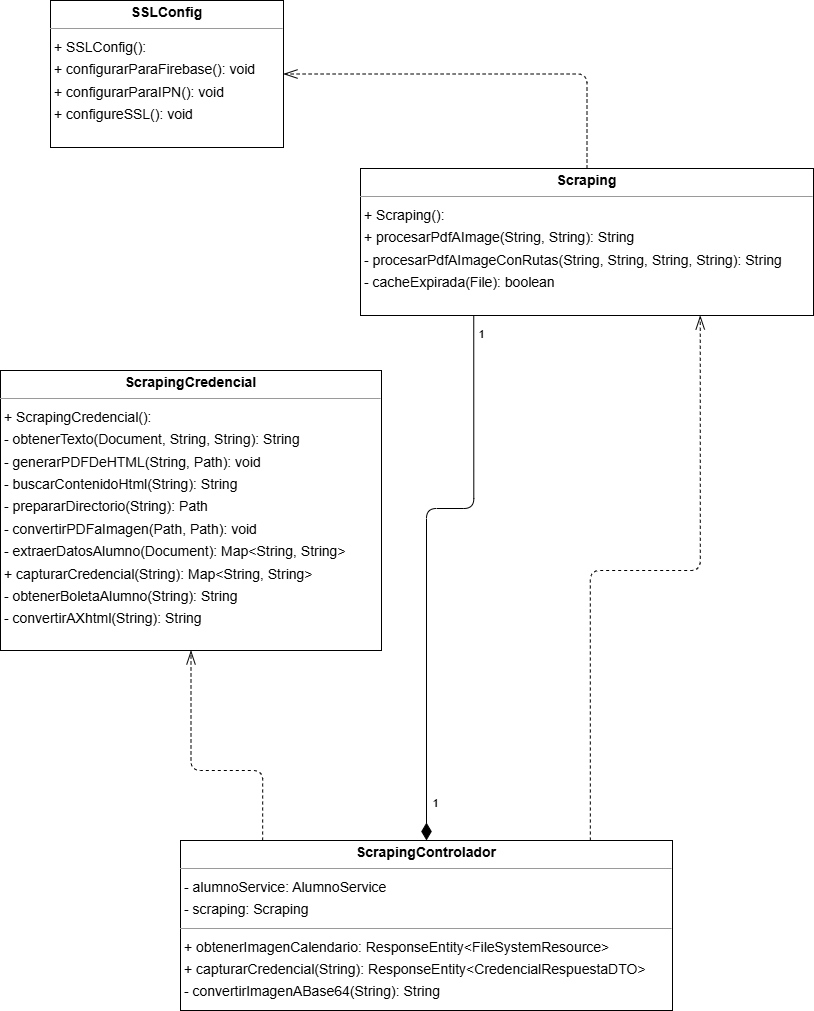
\includegraphics[width=0.9\textwidth]{Clases/Controlador5.png}
		\caption{Diagrama de clases de los controladores del servidor parte 5.}
		\label{fig:DC5}
	\end{center}
\end{figure}

\section{Estructura Interna Detallada de la Aplicación Móvil} 

La Figura \ref{fig:Diagrama_app_movil_detallado} profundiza en la arquitectura interna de la aplicación móvil, presentando los paquetes y componentes clave que la conforman. 

El punto de entrada principal de la aplicación es la actividad `MainActivity.kt`, la cual orquesta el flujo general de la aplicación. 

La interfaz de usuario de la aplicación se construye dentro del paquete `Pantallas`. Este paquete contiene las implementaciones de las pantallas de la aplicación utilizando Jetpack Compose. Cada pantalla se define mediante funciones Composable, que describen la estructura y el comportamiento de la interfaz de usuario de manera declarativa. 

La lógica y la gestión del estado de las `Pantallas` se encuentran en el paquete llamado `com.example.prueba3.Views`. Dentro de este paquete, los ViewModels actúan como intermediarios, proporcionando los datos necesarios a las Composables y manejando la lógica de las interacciones del usuario. Existe una relación directa entre las `Pantallas` y los `Views`, donde cada pantalla suele estar asociada a un ViewModel específico. 

El modelo de datos de la aplicación se define principalmente en el paquete `com.example.prueba3.Clases`. Este paquete contiene las clases que representan los datos utilizados por la aplicación. En su mayoría, estas clases son Data Classes, diseñadas para almacenar y transportar datos de manera concisa y eficiente.

La comunicación con los servicios backend se gestiona a través del paquete `RetroFit`. Este paquete contiene las interfaces de Retrofit que definen los endpoints de la API de los servidores remotos. Estas interfaces especifican las operaciones HTTP (GET, POST y DELETE) necesarias para interactuar con el Servidor Java Spring-Boot y el Servidor Red Neuronal. Retrofit se encarga de generar el código necesario para realizar estas solicitudes y procesar las respuestas del servidor.

\newpage

\begin{figure}[htbp!]
	\begin{center}
		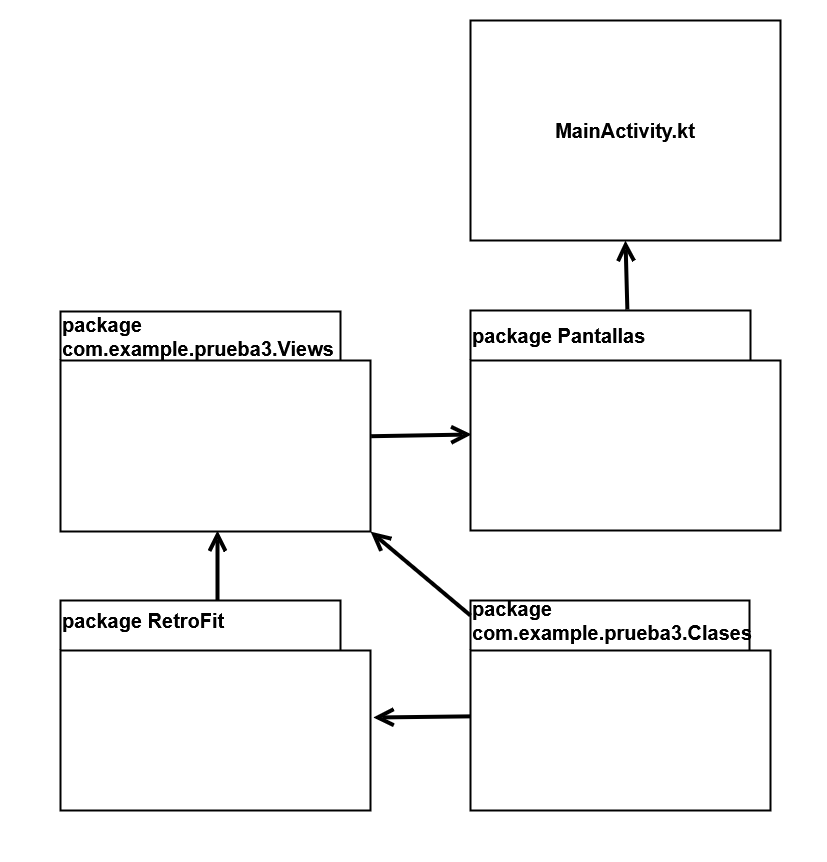
\includegraphics[width=0.6\textwidth]{DiagramasMoviles/DCM (1)}
		\caption{Estructura Interna Detallada de la Aplicación Móvil por Paquetes.}
		\label{fig:Diagrama_app_movil_detallado}
	\end{center}
\end{figure}



A continuación, se presentarán las clases contenidas en los paquetes `com.example.prueba3.Views` (ViewModels), `com.example.prueba3.Clases` (Data Classes) y las interfaces definidas en el paquete `RetroFit`, detallando su estructura y funcionalidad sección por sección. Adicionalmente, se incluirán diagramas de componentes específicos para cada una de las `Pantallas` de la aplicación móvil, ilustrando la composición de sus elementos y sus dependencias internas.

\newpage

\subsection{Diagramas de Componentes de package Pantallas}

Para una comprensión más profunda de la arquitectura de la interfaz de usuario de la aplicación móvil, a continuación se presentan los diagramas de componentes para cada una de las pantallas principales. Estos diagramas ilustran la composición interna de cada pantalla, mostrando los elementos de la interfaz de usuario (Composables), los datos que manejan y las posibles interacciones o dependencias con otros componentes. Cada diagrama proporciona una vista modular de la pantalla, facilitando la visualización de cómo se construyen las distintas secciones de la interfaz de usuario y cómo se relacionan entre sí. La Figura \ref{fig:Pantallas} muestra las pantallas (archivos .kt) presentes en package.Pantallas.

\begin{figure}[htbp!]
	\begin{center}
		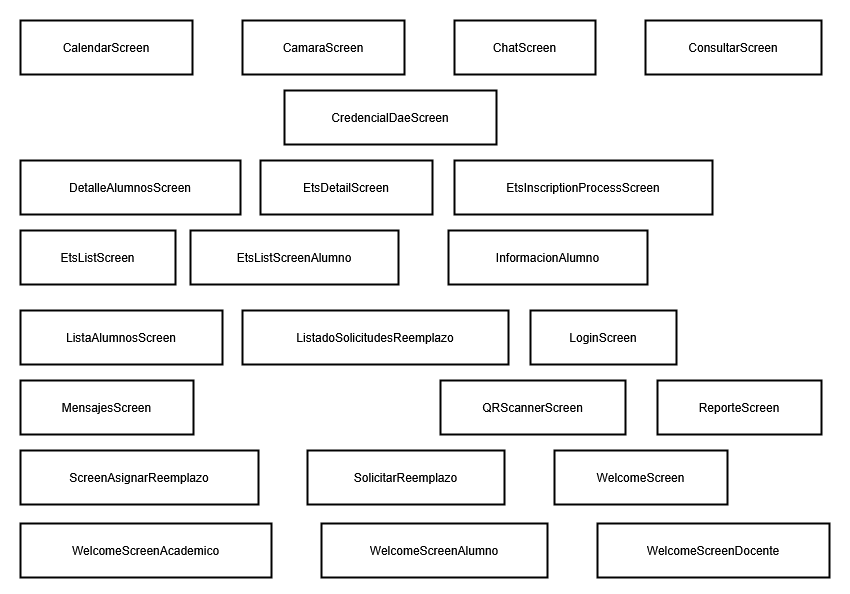
\includegraphics[width=0.9\textwidth]{DiagramasMoviles/DCM (12)}
		\caption{Pantallas presentes en package.Pantallas (archivos .kt).}
		\label{fig:Pantallas}
	\end{center}
\end{figure}


\newpage

\subsection{Diagrama de Componentes de CalendarScreen.kt}

La Figura \ref{fig:Componentes_1} muestra el diagrama de componentes para CalendarScreen.kt que es un composable que contiene a la \IUref{IU02}{Pantalla Consultar calendario escolar}, que muestra el calendario escolar y permite al usuario ver cuantos días faltan para el periodo de ETS próximo si esta disponible.

\begin{figure}[htbp!]
	\begin{center}
		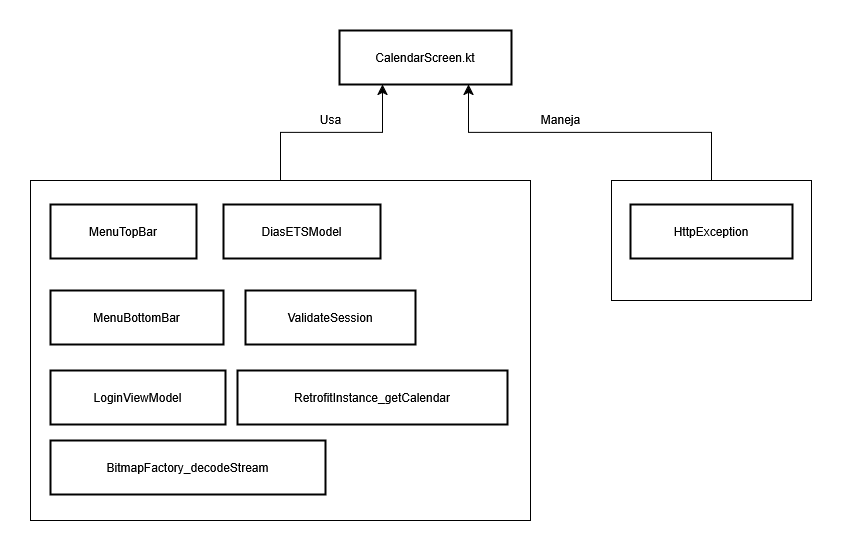
\includegraphics[width=0.9\textwidth]{DiagramasMoviles/DCM (13)}
		\caption{Diagrama de componentes para CalendarScreen.kt .}
		\label{fig:Componentes_1}
	\end{center}
\end{figure}

\newpage

\subsection{Diagrama de Componentes de CamaraScreen.kt}

La Figura \ref{fig:Componentes_2} muestra el diagrama de componentes para CamaraScreen.kt que es un composable que contiene a la \IUref{IU17}{Pantalla de Reconocimiento facial} y la \IUref{IU19}{Pantalla de Reconocimiento facial alumno}, que muestran la cámara usada para obtener la foto que se usara para el proceso de reconocimiento facial.

\begin{figure}[htbp!]
	\begin{center}
		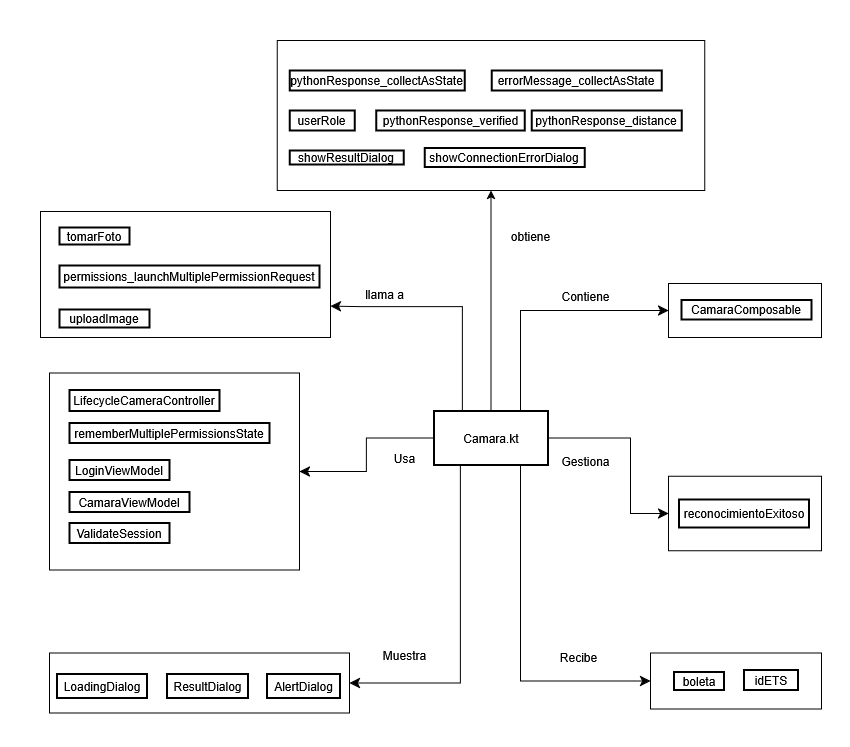
\includegraphics[width=0.9\textwidth]{DiagramasMoviles/DCM (14)}
		\caption{Diagrama de componentes para CamaraScreen.kt .}
		\label{fig:Componentes_2}
	\end{center}
\end{figure}

\newpage

\subsection{Diagrama de Componentes de ChatScreen.kt}

La Figura \ref{fig:Componentes_3} muestra el diagrama de componentes para ChatScreen.kt que es un composable que contiene una pantalla que muestra el chat de mensajes que pueden usar los usuarios.

\begin{figure}[htbp!]
	\begin{center}
		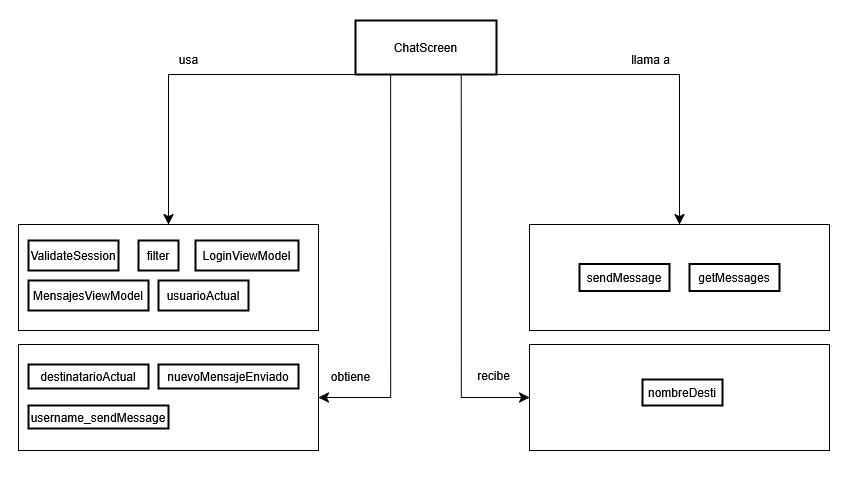
\includegraphics[width=0.9\textwidth]{DiagramasMoviles/DCM (15)}
		\caption{Diagrama de componentes para ChatScreen.kt .}
		\label{fig:Componentes_3}
	\end{center}
\end{figure}

\newpage

\subsection{Diagrama de Componentes de ConsultarScreen.kt}

La Figura \ref{fig:Componentes_4} muestra el diagrama de componentes para ConsultarScreen.kt que es un composable que contiene a la \IUref{IU12}{Pantalla Buscar alumno}, que muestra la lista de los alumnos inscritos a un ETS para el personal de seguridad y le permite filtrarlos por nombre o boleta.

\begin{figure}[htbp!]
	\begin{center}
		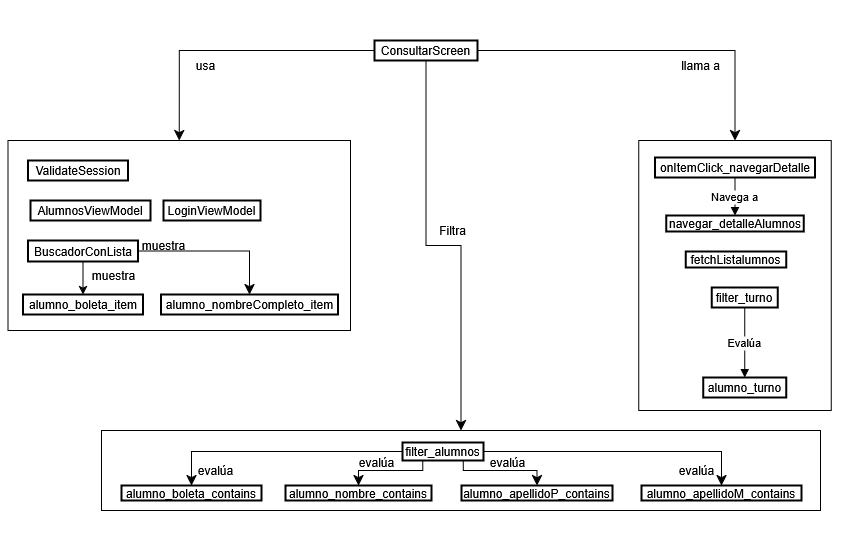
\includegraphics[width=0.9\textwidth]{DiagramasMoviles/DCM (16)}
		\caption{Diagrama de componentes para ConsultarScreen.kt .}
		\label{fig:Componentes_4}
	\end{center}
\end{figure}

\newpage

\subsection{Diagrama de Componentes de CredencialDaeScreen.kt}

La Figura \ref{fig:Componentes_5} muestra el diagrama de componentes para CredencialDaeScreen.kt que es un composable que contiene a la \IUref{IU11}{Pantalla Credencial del alumno}, que muestra la comparación de la credencial de la DAE con la credencial creada por el sistema.

\begin{figure}[htbp!]
	\begin{center}
		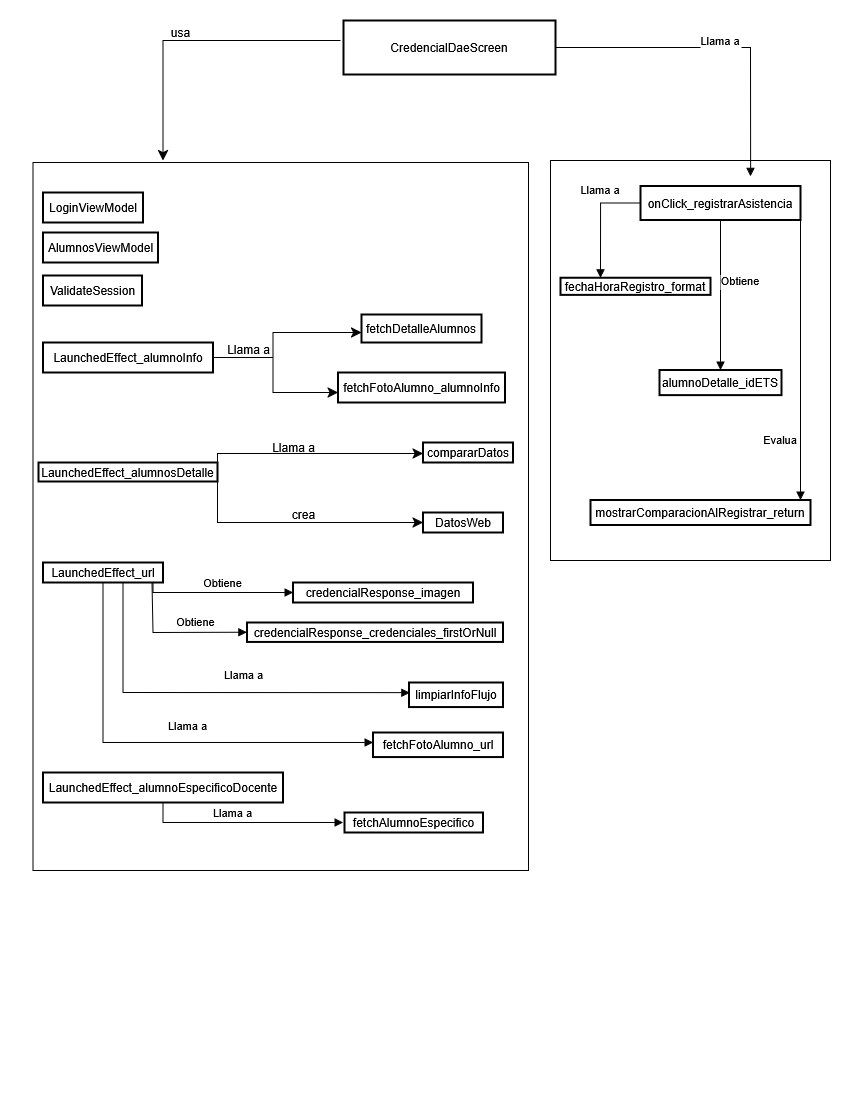
\includegraphics[width=0.9\textwidth]{DiagramasMoviles/DCM (17)}
		\caption{Diagrama de componentes para CredencialDaeScreen.kt .}
		\label{fig:Componentes_5}
	\end{center}
\end{figure}

\newpage

\subsection{Diagrama de Componentes de DetallesAlumnosScreen.kt}

La Figura \ref{fig:Componentes_6} muestra el diagrama de componentes para DetallesAlumnosScreen.kt que es un composable que contiene a la \IUref{IU11}{Pantalla Credencial del alumno}, que en este caso muestra la información relevante del alumno.

\begin{figure}[htbp!]
	\begin{center}
		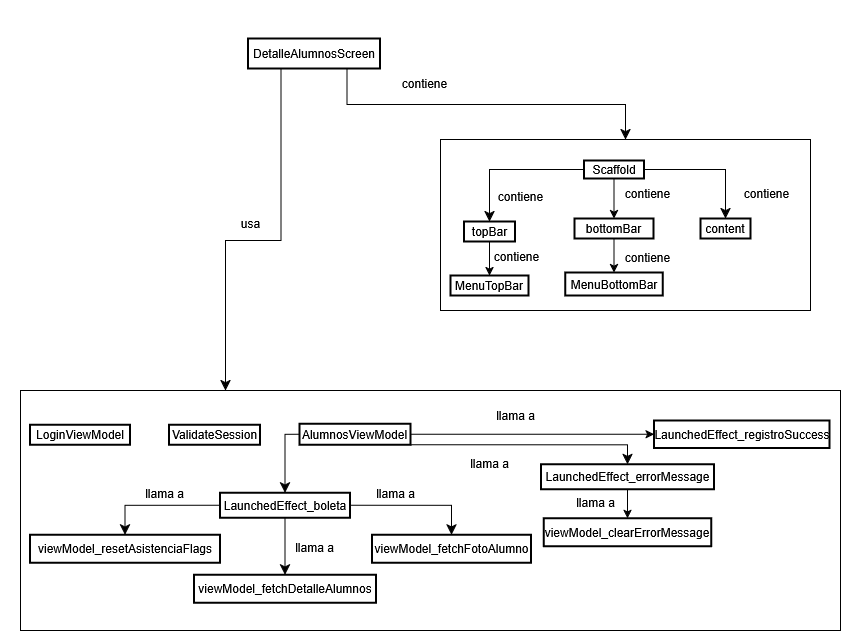
\includegraphics[width=0.9\textwidth]{DiagramasMoviles/DCM (19)}
		\caption{Diagrama de componentes para DetallesAlumnosScreen.kt .}
		\label{fig:Componentes_6}
	\end{center}
\end{figure}

\newpage

\subsection{Diagrama de Componentes de EtsDetailScreen.kt}

La Figura \ref{fig:Componentes_7} muestra el diagrama de componentes para EtsDetailScreen.kt que es un composable que contiene a la \IUref{IU06}{Pantalla Información de ETS} y \IUref{IU16}{Pantalla Información de ETS del alumno}, que muestra la información del ETS elegido por el usuario.

\begin{figure}[htbp!]
	\begin{center}
		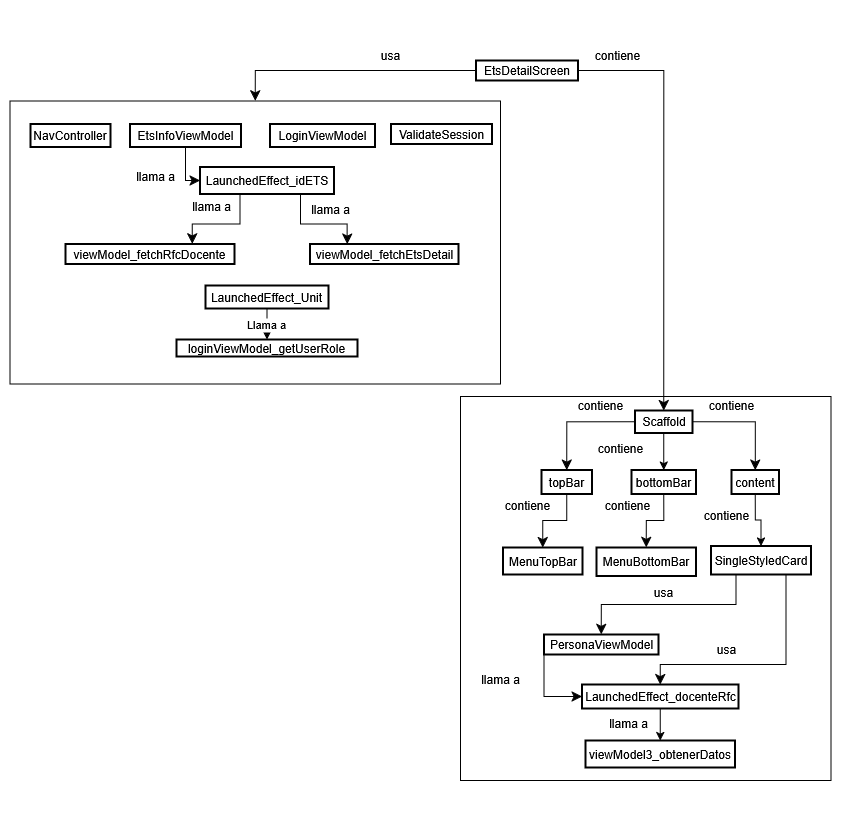
\includegraphics[width=0.9\textwidth]{DiagramasMoviles/DCM (20)}
		\caption{Diagrama de componentes para EtsDetailScreen.kt .}
		\label{fig:Componentes_7}
	\end{center}
\end{figure}

\newpage

\subsection{Diagrama de Componentes de EtsInscriptionProcessScreen.kt}

La Figura \ref{fig:Componentes_8} muestra el diagrama de componentes para ETSInscriptionProcessScreen.kt que es un composable que contiene a la \IUref{IU18}{Pantalla de Detalles del proceso de ETS}, que muestra la información necesaria para inscribirse a un ETS.

\begin{figure}[htbp!]
	\begin{center}
		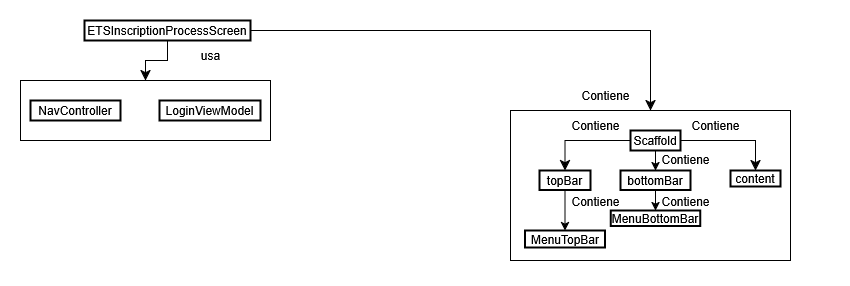
\includegraphics[width=0.9\textwidth]{DiagramasMoviles/DCM (21)}
		\caption{Diagrama de componentes para ETSInscriptionProcessScreen.kt .}
		\label{fig:Componentes_8}
	\end{center}
\end{figure}

\newpage

\subsection{Diagrama de Componentes de EtsListScreen.kt}

La Figura \ref{fig:Componentes_9} muestra el diagrama de componentes para EtsListScreen.kt que es un composable que contiene a la \IUref{IU05}{Pantalla Consultar ETS}, que muestra la lista de ETS del docente.

\begin{figure}[htbp!]
	\begin{center}
		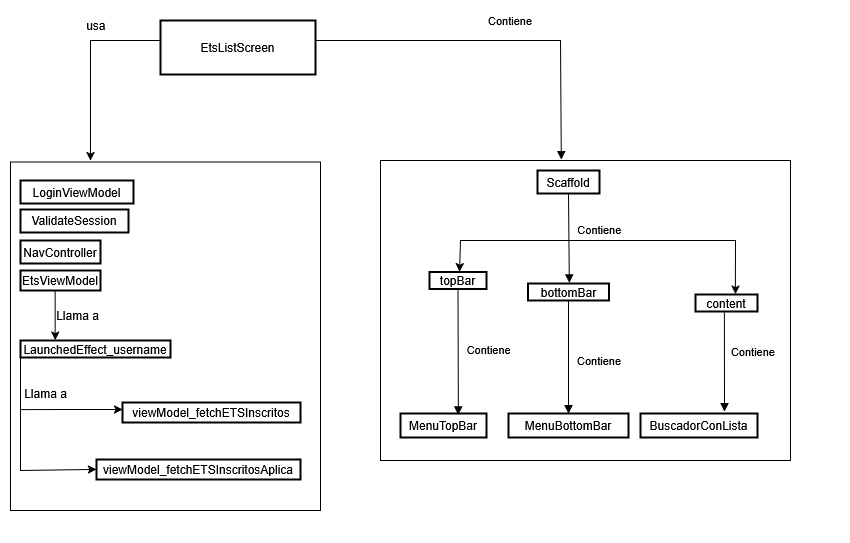
\includegraphics[width=0.9\textwidth]{DiagramasMoviles/DCM (22)}
		\caption{Diagrama de componentes para EtsListScreen.kt .}
		\label{fig:Componentes_9}
	\end{center}
\end{figure}

\newpage

\subsection{Diagrama de Componentes de EtsListScreenAlumno.kt}

La Figura \ref{fig:Componentes_10} muestra el diagrama de componentes para EtsListScreenAlumno.kt que es un composable que contiene a la \IUref{IU05}{Pantalla Consultar ETS}, que muestra la lista de ETS del alumno.

\begin{figure}[htbp!]
	\begin{center}
		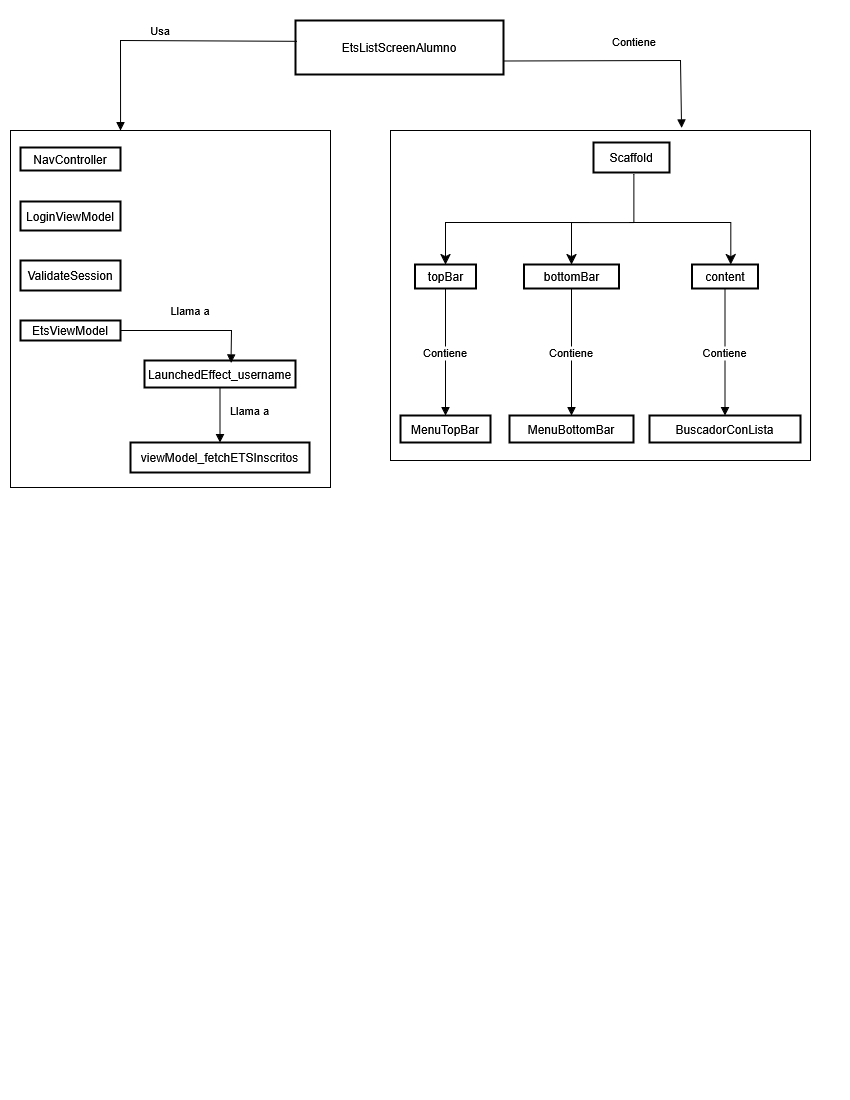
\includegraphics[width=0.9\textwidth]{DiagramasMoviles/DCM (23)}
		\caption{Diagrama de componentes para EtsListScreenAlumno.kt .}
		\label{fig:Componentes_10}
	\end{center}
\end{figure}

\newpage

\subsection{Diagrama de Componentes de InformacionAlumno.kt}

La Figura \ref{fig:Componentes_11} muestra el diagrama de componentes para InformacionAlumno.kt que es un composable que contiene a la \IUref{IUE07}{Creación del reporte}, que se utiliza para la creación de reportes y a su vez muestra la información esencial del alumno seleccionado.

\begin{figure}[htbp!]
	\begin{center}
		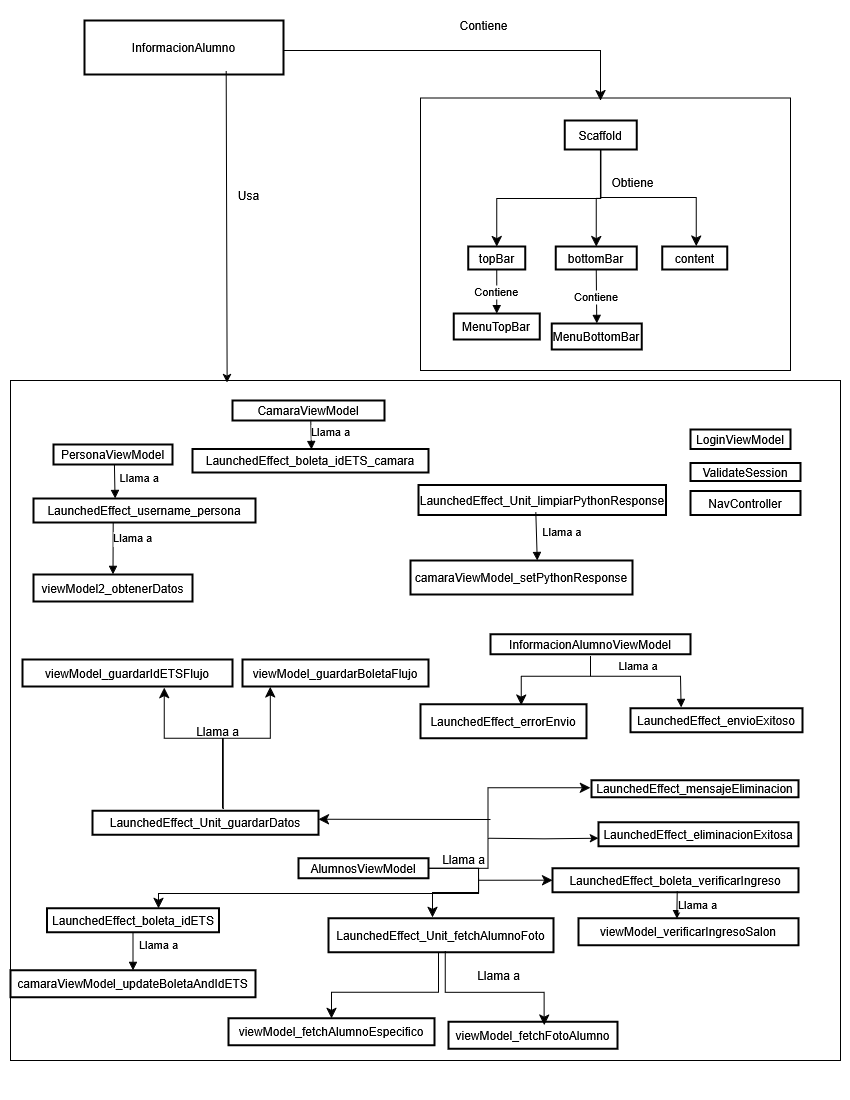
\includegraphics[width=0.7\textwidth]{DiagramasMoviles/DCM (24)}
		\caption{Diagrama de componentes para InformacionAlumno.kt .}
		\label{fig:Componentes_11}
	\end{center}
\end{figure}

\newpage

\subsection{Diagrama de Componentes de ListaAlumnosScreen.kt}

La Figura \ref{fig:Componentes_12} muestra el diagrama de componentes para ListaAlumnosScreen.kt que es un composable que contiene a la \IUref{IU08}{Pantalla Lista de asistencia de ETS}, que es la que le muestra la lista de alumnos inscritos a un ETS al docente, junto con su estado de asistencia con un icono.

\begin{figure}[htbp!]
	\begin{center}
		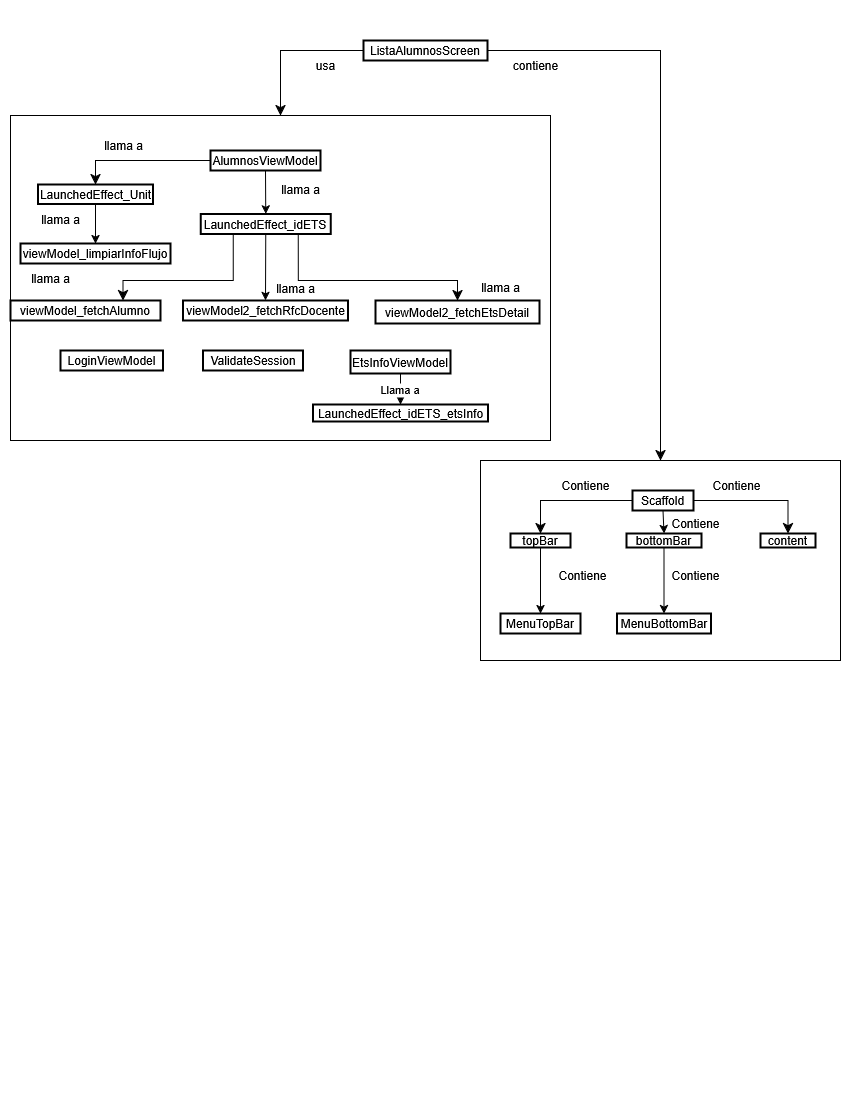
\includegraphics[width=0.9\textwidth]{DiagramasMoviles/DCM (25)}
		\caption{Diagrama de componentes para ListaAlumnosScreen.kt .}
		\label{fig:Componentes_12}
	\end{center}
\end{figure}

\newpage

\subsection{Diagrama de Componentes de ListadoSolicitudesReemplazo.kt}

La Figura \ref{fig:Componentes_13} muestra el diagrama de componentes para ListadoSolicitudesReemplazo.kt que es un composable que contiene una pantalla dedica a la visualización de las solicitudes de reemplazo y sus estados de aceptación o denegación. 

\begin{figure}[htbp!]
	\begin{center}
		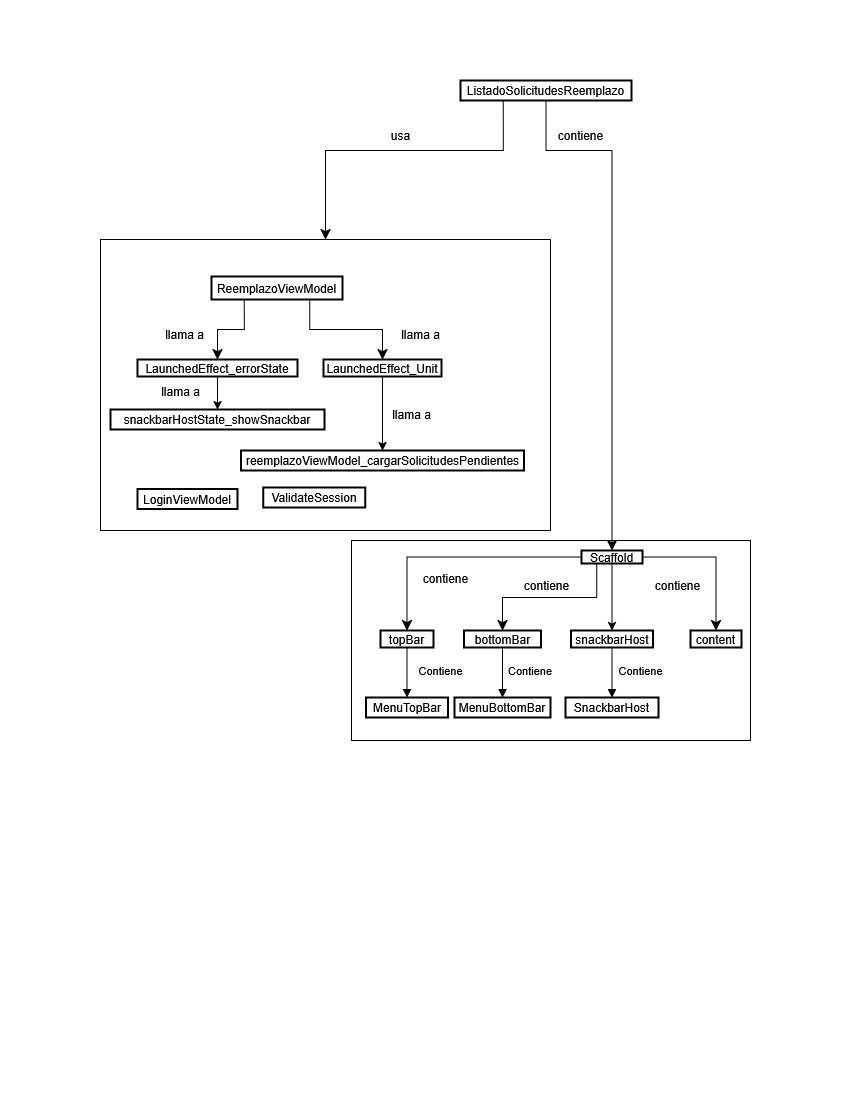
\includegraphics[width=0.9\textwidth]{DiagramasMoviles/DCM (26)}
		\caption{Diagrama de componentes para ListadoSolicitudesReemplazo.kt .}
		\label{fig:Componentes_13}
	\end{center}
\end{figure}

\newpage

\subsection{Diagrama de Componentes de LoginScreen.kt}

La Figura \ref{fig:Componentes_14} muestra el diagrama de componentes para LoginScreen.kt que es un composable que contiene a la \IUref{IU01}{Pantalla Iniciar sesión del sistema móvil}, que es el login de la aplicación móvil.

\begin{figure}[htbp!]
	\begin{center}
		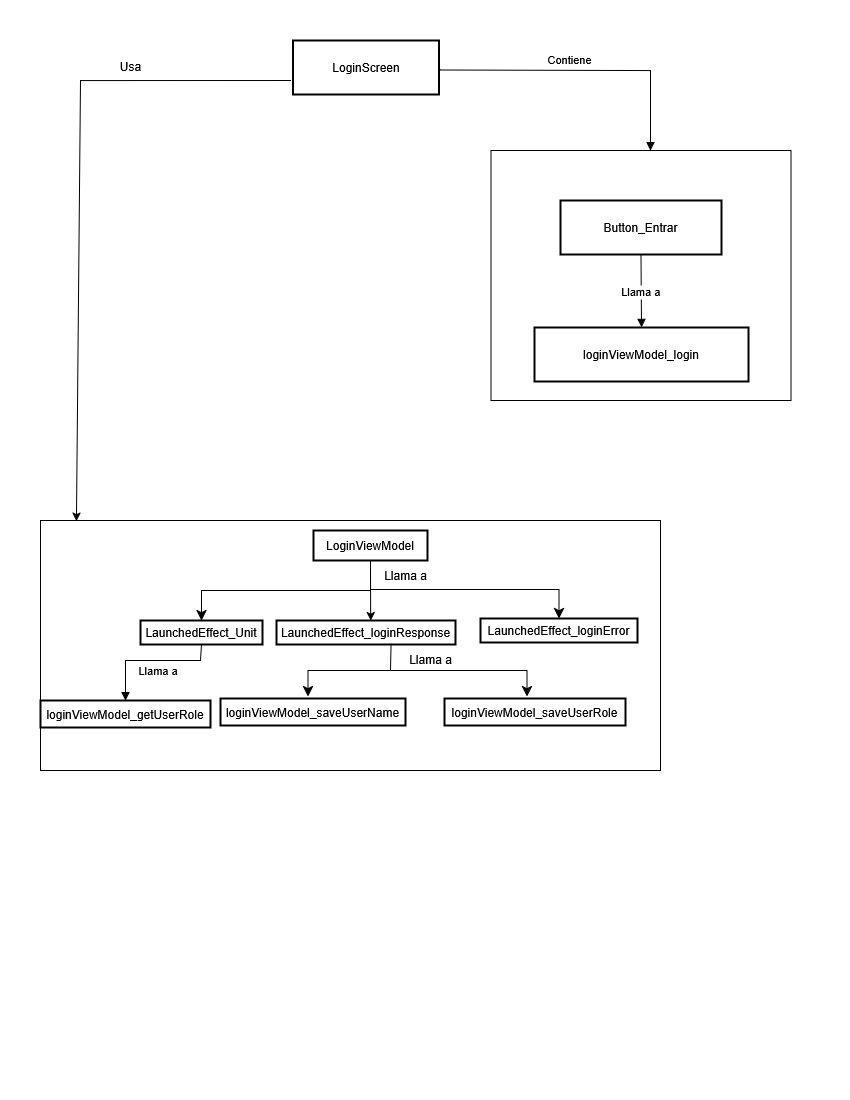
\includegraphics[width=0.9\textwidth]{DiagramasMoviles/DCM (27)}
		\caption{Diagrama de componentes para LoginScreen.kt .}
		\label{fig:Componentes_14}
	\end{center}
\end{figure}

\newpage

\subsection{Diagrama de Componentes de MensajesScreen.kt}

La Figura \ref{fig:Componentes_15} muestra el diagrama de componentes para MensajesScreen.kt que es un composable que es la pantalla donde se ven los mensaje específicos mandados a otro usuario.

\begin{figure}[htbp!]
	\begin{center}
		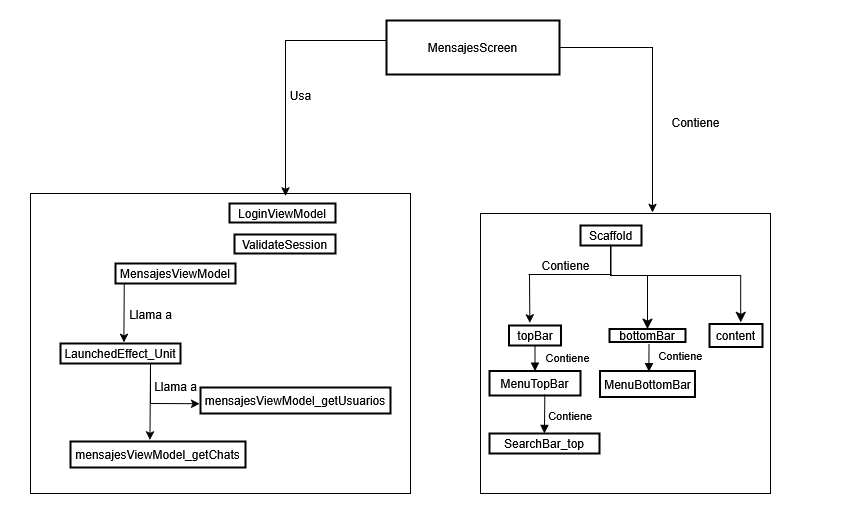
\includegraphics[width=0.9\textwidth]{DiagramasMoviles/DCM (28)}
		\caption{Diagrama de componentes para MensajesScreen.kt .}
		\label{fig:Componentes_15}
	\end{center}
\end{figure}

\newpage

\subsection{Diagrama de Componentes de QRScannerScreen.kt}

La Figura \ref{fig:Componentes_16} muestra el diagrama de componentes para QRScannerScreen.kt que es un composable que contiene a la \IUref{IU10}{Pantalla Código QR}, que muestra la cámara para poder escanear el código QR de la credencial del alumno.

\begin{figure}[htbp!]
	\begin{center}
		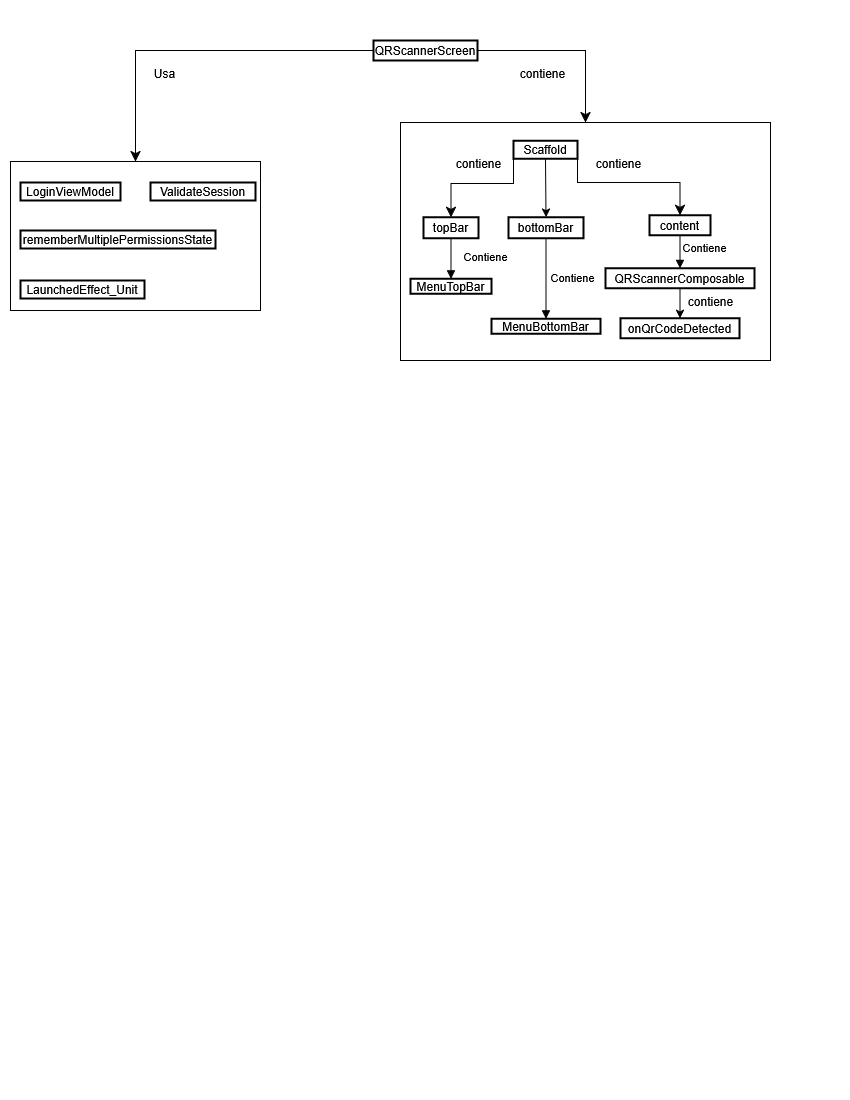
\includegraphics[width=0.9\textwidth]{DiagramasMoviles/DCM (29)}
		\caption{Diagrama de componentes para QRScannerScreen.kt .}
		\label{fig:Componentes_16}
	\end{center}
\end{figure}

\newpage

\subsection{Diagrama de Componentes de ReporteScreen.kt}

La Figura \ref{fig:Componentes_17} muestra el diagrama de componentes para ReporteScreen.kt que es un composable que contiene a la \IUref{IU20}{Pantalla Reporte del Alumno}, que es donde el docente puede revisar el reporte de la asistencia del alumno.

\begin{figure}[htbp!]
	\begin{center}
		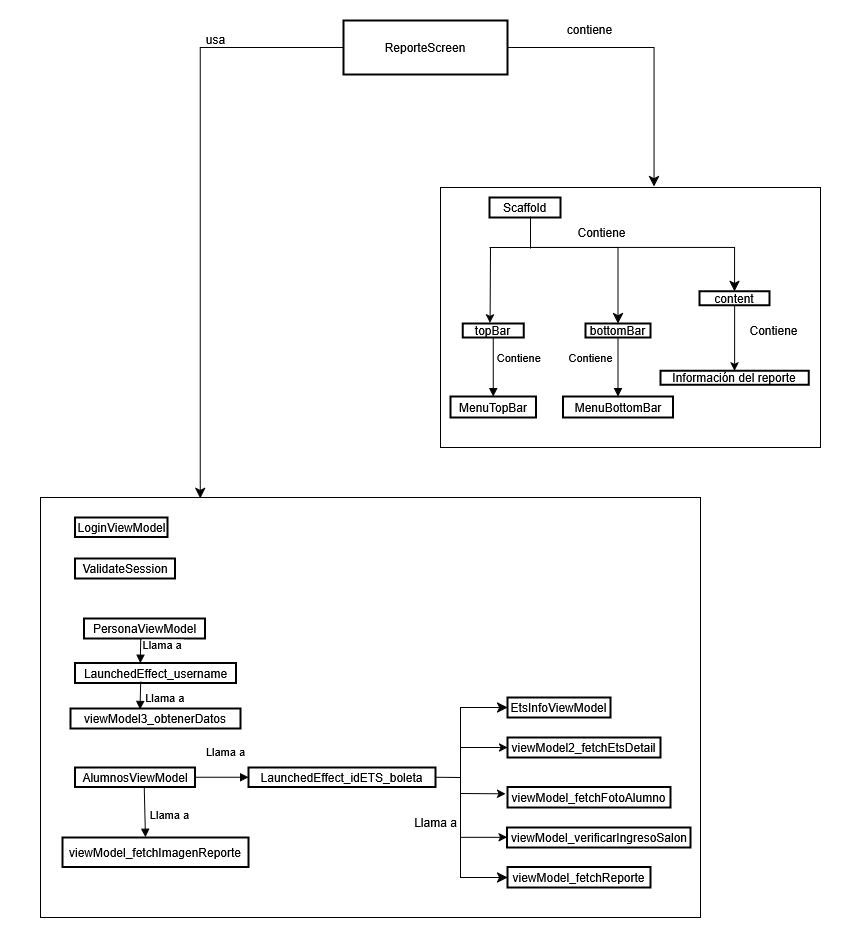
\includegraphics[width=0.7\textwidth]{DiagramasMoviles/DCM (30)}
		\caption{Diagrama de componentes para ReporteScreen.kt .}
		\label{fig:Componentes_17}
	\end{center}
\end{figure}

\newpage

\subsection{Diagrama de Componentes de ScreenAsignarremplazo.kt}

La Figura \ref{fig:Componentes_18} muestra el diagrama de componentes para ScreenAsignarremplazo.kt que es un composable que contiene a la pantalla \IUref{IU09}{Asignar docente de remplazo}, que es donde el jefe de departamento y/o el presidente de academia pueden responder a las solicitudes de reemplazo.

\begin{figure}[htbp!]
	\begin{center}
		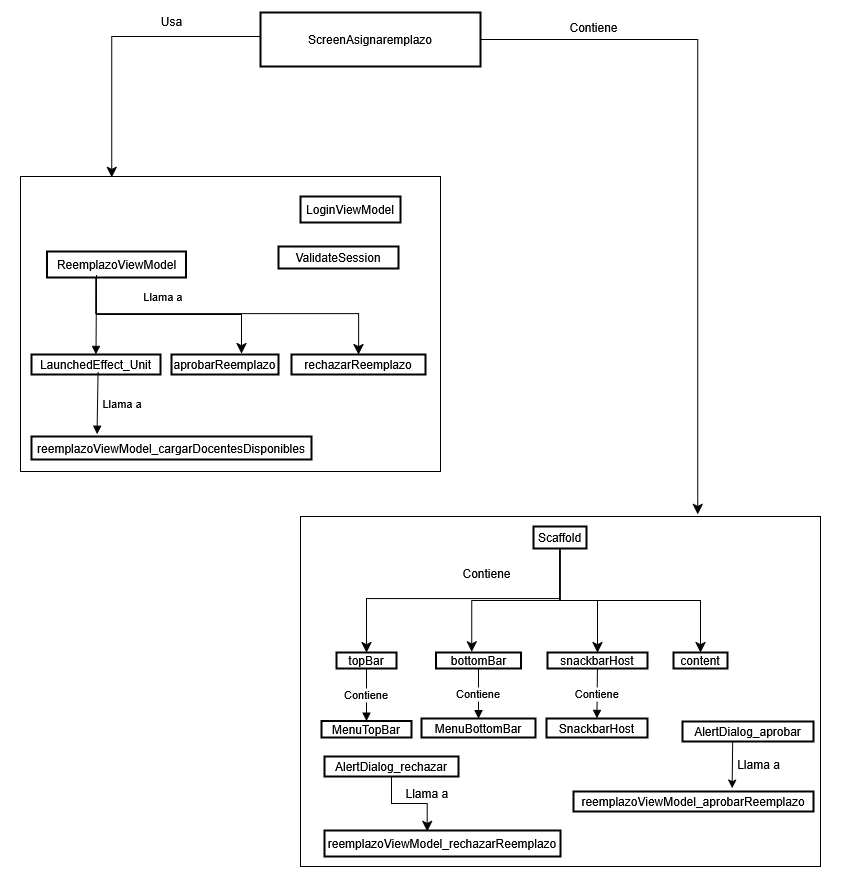
\includegraphics[width=0.9\textwidth]{DiagramasMoviles/DCM (31)}
		\caption{Diagrama de componentes para ScreenAsignarremplazo.kt .}
		\label{fig:Componentes_18}
	\end{center}
\end{figure}

\newpage

\subsection{Diagrama de Componentes de SolicitarReemplazo.kt}

La Figura \ref{fig:Componentes_19} muestra el diagrama de componentes para SolicitarReemplazo.kt que es un composable que contiene a la \IUref{IU07}{Pantalla de Solicitar remplazo}, que es donde el docente puede pedir un reemplazo como aplacador del ETS.

\begin{figure}[htbp!]
	\begin{center}
		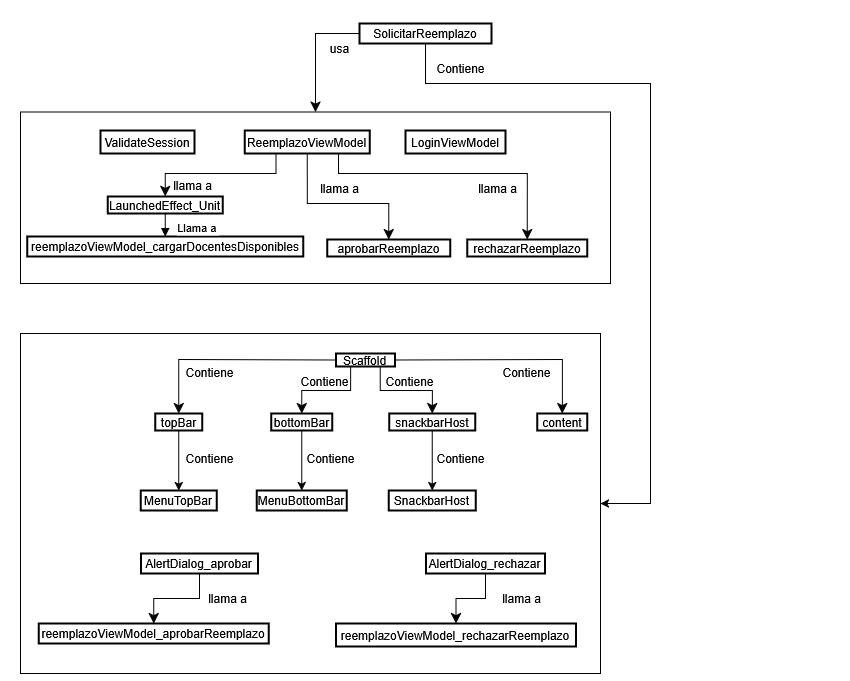
\includegraphics[width=0.9\textwidth]{DiagramasMoviles/DCM (32)}
		\caption{Diagrama de componentes para SolicitarReemplazo.kt .}
		\label{fig:Componentes_19}
	\end{center}
\end{figure}

\newpage

\subsection{Diagrama de Componentes de WelcomeScreen.kt}

La Figura \ref{fig:Componentes_20} muestra el diagrama de componentes para WelcomeScreen.kt que es un composable que contiene a la \IUref{IUE02}{Pantalla de saludo del personal de seguridad}, que es la pantalla de inicio del personal de seguridad (donde pude seleccionar la operación que quiere realizar y ver un saludo con su nombre).

\begin{figure}[htbp!]
	\begin{center}
		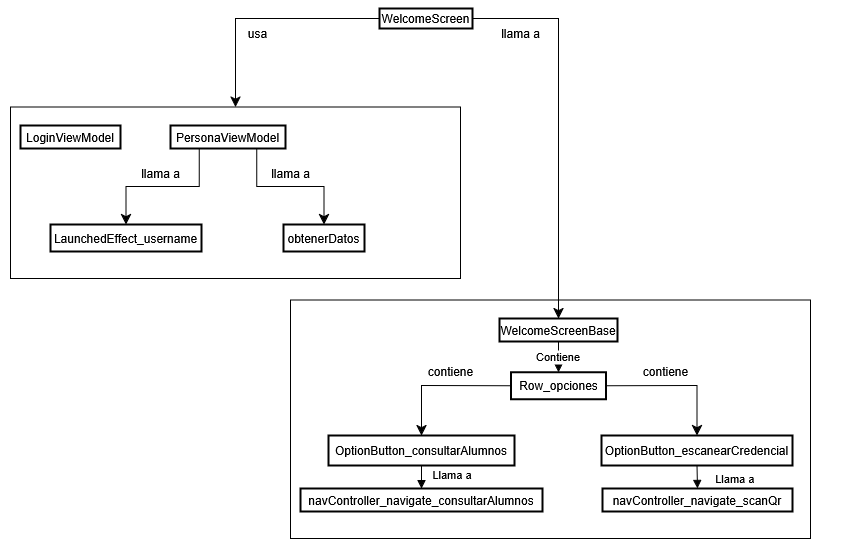
\includegraphics[width=0.9\textwidth]{DiagramasMoviles/DCM (33)}
		\caption{Diagrama de componentes para WelcomeScreen.kt .}
		\label{fig:Componentes_20}
	\end{center}
\end{figure}

\newpage

\subsection{Diagrama de Componentes de WelcomeScreenAcademico.kt}

La Figura \ref{fig:Componentes_21} muestra el diagrama de componentes para WelcomeScreenAcademico.kt que es un composable que contiene a la pantalla \IUref{IUE06}{saludo del presidente de academia y el jefe de departamento}, que es la pantalla de inicio del jefe de departamento y/o el presidente de academia (donde pude seleccionar la operación que quiere realizar y ver un saludo con su nombre).

\begin{figure}[htbp!]
	\begin{center}
		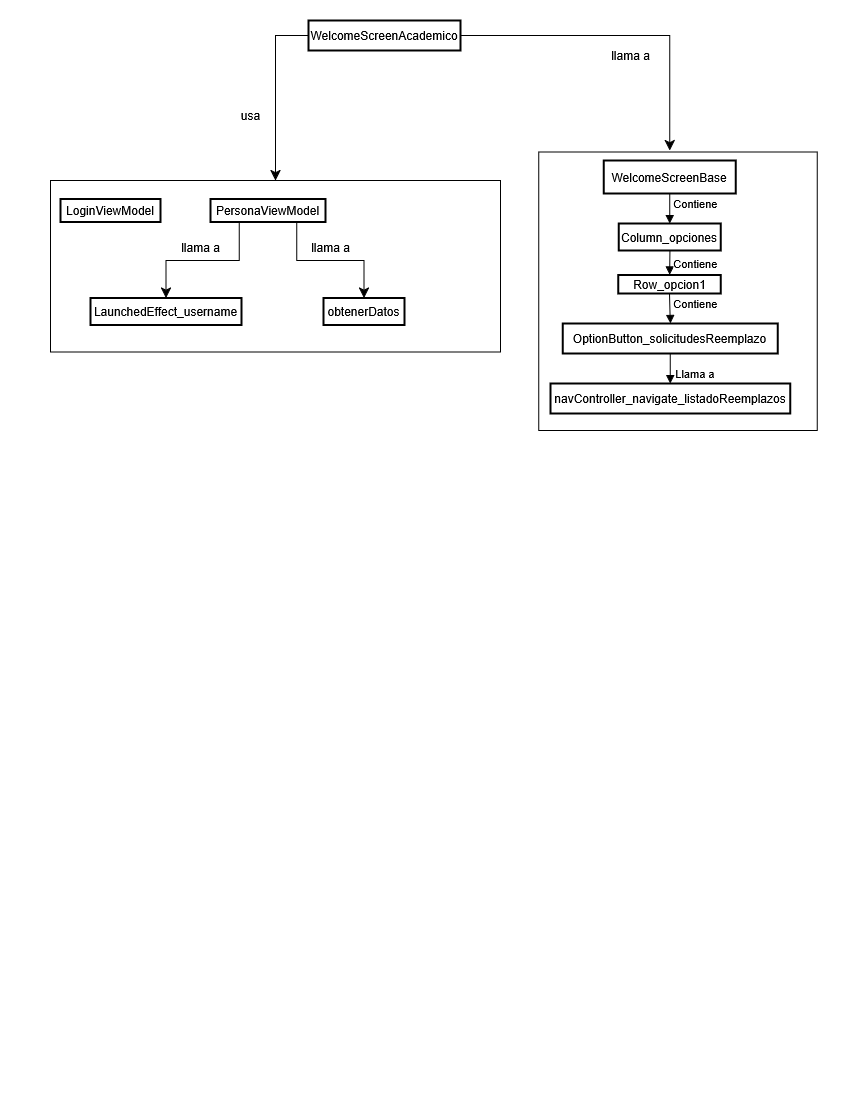
\includegraphics[width=0.9\textwidth]{DiagramasMoviles/DCM (34)}
		\caption{Diagrama de componentes para WelcomeScreenAcademico.kt .}
		\label{fig:Componentes_21}
	\end{center}
\end{figure}

\newpage

\subsection{Diagrama de Componentes de WelcomeScreenAlumno.kt}

La Figura \ref{fig:Componentes_22} muestra el diagrama de componentes para WelcomeScreenAlumno.kt que es un composable que contiene a la pantalla \IUref{IUE03}{Pantalla saludo del alumno}, que es la pantalla de inicio del Alumno (donde pude seleccionar la operación que quiere realizar y ver un saludo con su nombre).

\begin{figure}[htbp!]
	\begin{center}
		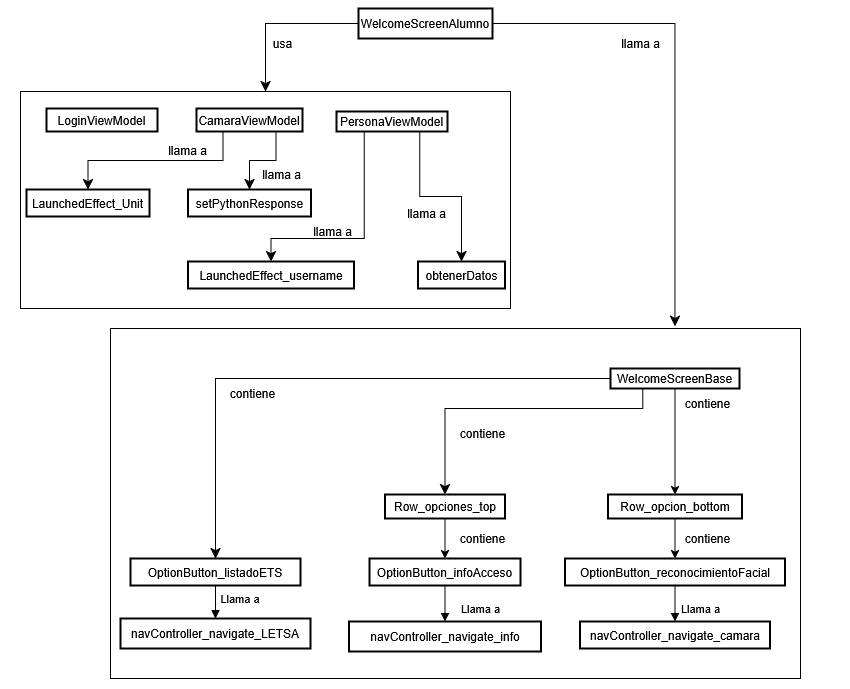
\includegraphics[width=0.9\textwidth]{DiagramasMoviles/DCM (35)}
		\caption{Diagrama de componentes para WelcomeScreenAlumno.kt .}
		\label{fig:Componentes_22}
	\end{center}
\end{figure}

\newpage

\subsection{Diagrama de Componentes de WelcomeScreenDocente.kt}

La Figura \ref{fig:Componentes_23} muestra el diagrama de componentes para WelcomeScreenDocente.kt que es un composable que contiene a la pantalla \IUref{IUE01}{Pantalla saludo de docente}, que es la pantalla de inicio del Docente (donde pude seleccionar la operación que quiere realizar y ver un saludo con su nombre).

\begin{figure}[htbp!]
	\begin{center}
		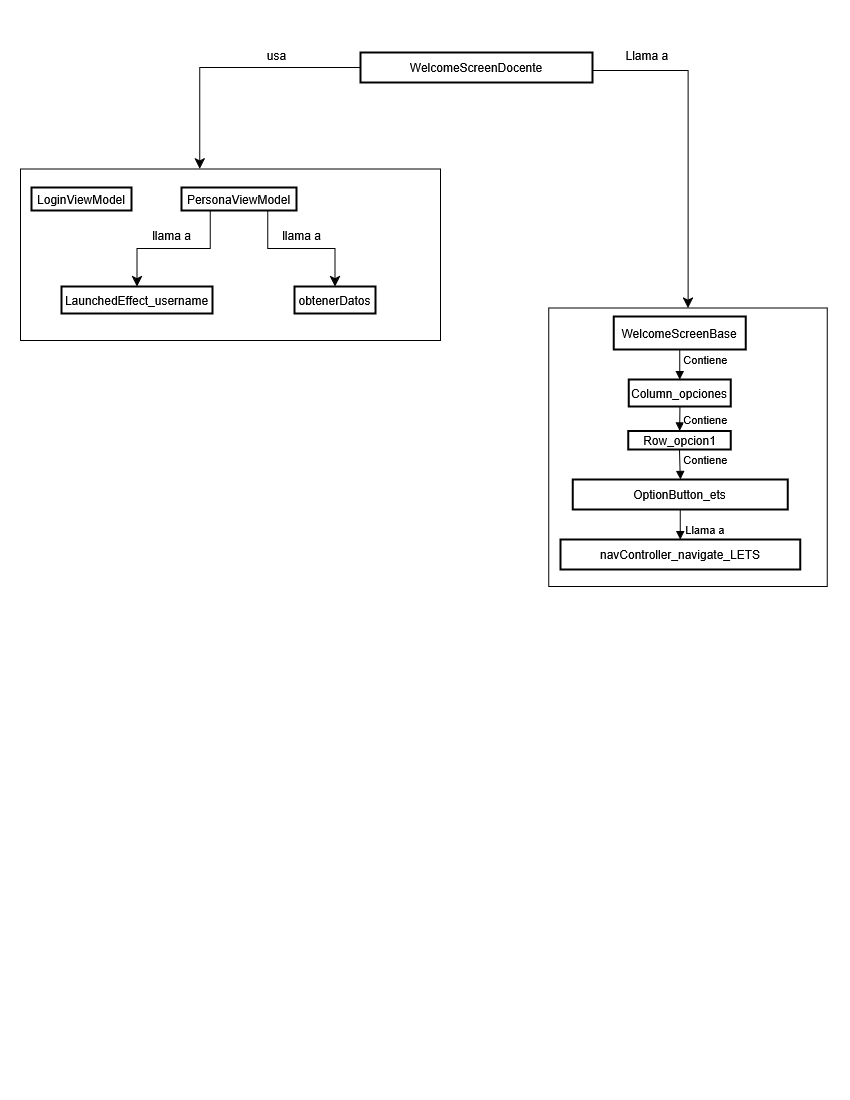
\includegraphics[width=0.8\textwidth]{DiagramasMoviles/DCM (36)}
		\caption{Diagrama de componentes para WelcomeScreenDocente.kt .}
		\label{fig:Componentes_23}
	\end{center}
\end{figure}

\subsection{Diagramas de clases de package com.example.prueba3.Views}

La arquitectura de nuestra aplicación móvil se organiza en paquetes bien definidos para una clara separación de responsabilidades. Dentro de este esquema, el paquete `com.example.prueba3.Views`, que contiene nuestros ViewModels, se erige como un componente central y fundamental.

Los ViewModels son elementos clave en la construcción de interfaces de usuario robustas y reactivas. Su función primordial es actuar como intermediarios estratégicos entre las `Pantallas` (implementadas como Composables en el paquete `Pantallas`), y la lógica de negocio o las fuentes de datos. Un ViewModel se encarga de exponer los datos necesarios para su `Pantalla` asociada de una manera que sea óptima para la interfaz de usuario, garantizando que el estado de la UI persista a través de cambios de configuración del dispositivo, como rotaciones o reconstrucciones de la actividad.

A continuación se presentara las clases que conforman a package.example.prueba3.Views:


\subsection{Diagrama de clases de package.example.prueba3.Views parte 1}

La Figura \ref{fig:Views1} muestra la primera parte del diagrama de clases de package.example.prueba3.Views.

\begin{figure}[htbp!]
	\begin{center}
		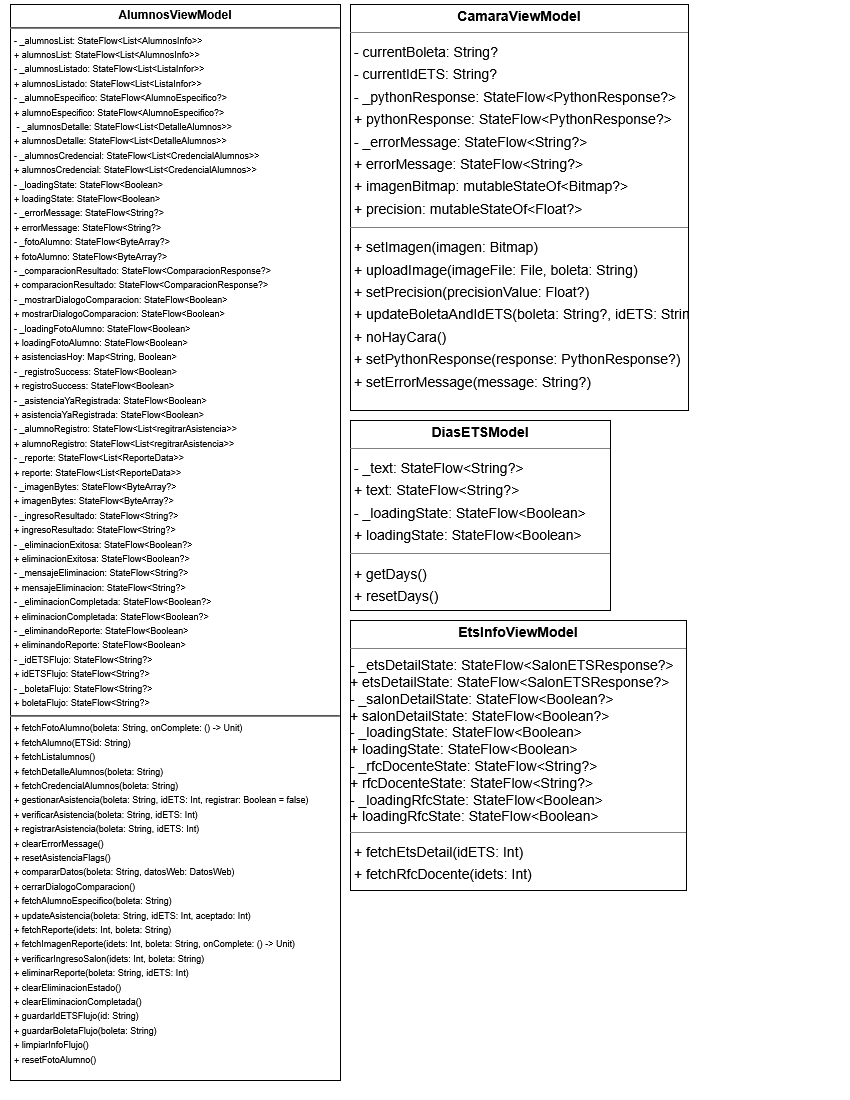
\includegraphics[width=0.75\textwidth]{DiagramasMoviles/DCM (7)}
		\caption{Diagrama de clases para package.example.prueba3.Views parte 1.}
		\label{fig:Views1}
	\end{center}
\end{figure}

\newpage

\subsection{Diagrama de clases de package.example.prueba3.Views parte 2}

La Figura \ref{fig:Views2} muestra la segunda parte del diagrama de clases de package.example.prueba3.Views.

\begin{figure}[htbp!]
	\begin{center}
		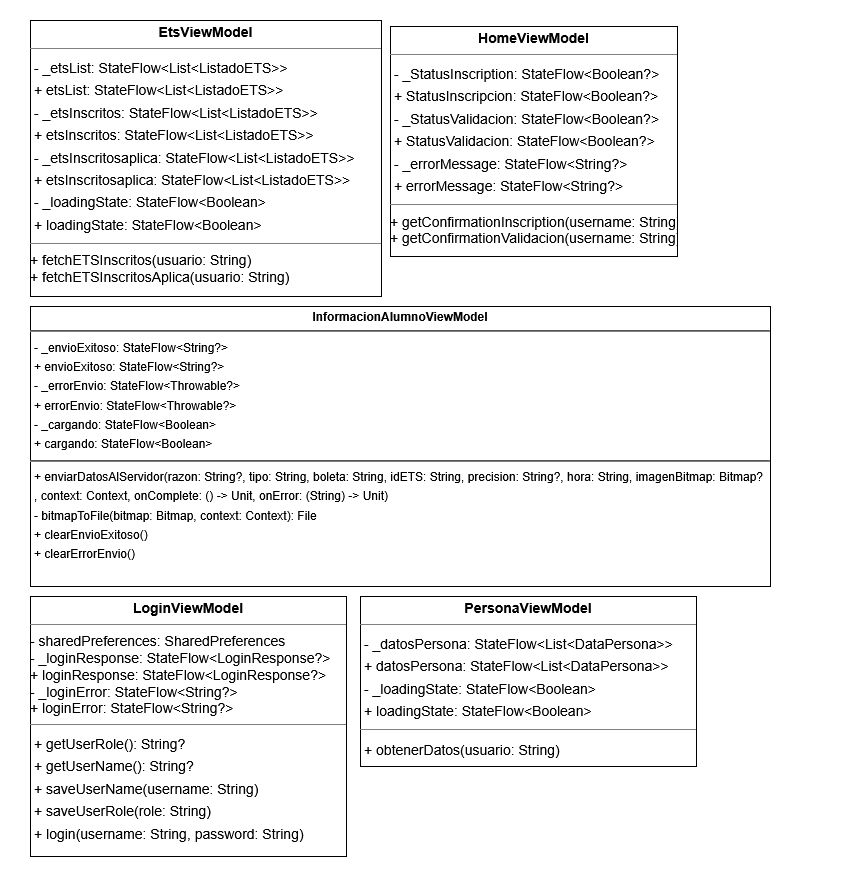
\includegraphics[width=0.75\textwidth]{DiagramasMoviles/DCM (8)}
		\caption{Diagrama de clases para package.example.prueba3.Views parte 2.}
		\label{fig:Views2}
	\end{center}
\end{figure}

\newpage

\subsection{Diagrama de clases de package.example.prueba3.Views parte 3}

La Figura \ref{fig:Views3} muestra la tercer parte del diagrama de clases de package.example.prueba3.Views.

\begin{figure}[htbp!]
	\begin{center}
		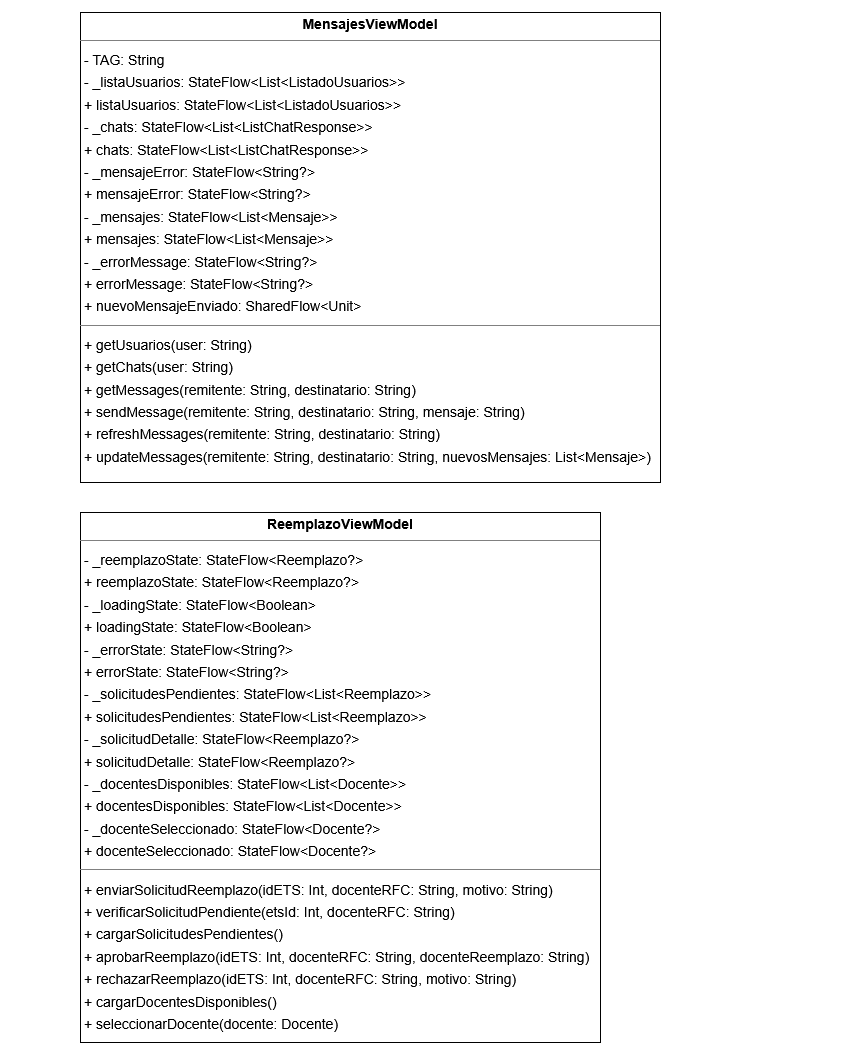
\includegraphics[width=0.75\textwidth]{DiagramasMoviles/DCM (9)}
		\caption{Diagrama de clases para package.example.prueba3.Views parte 3.}
		\label{fig:Views3}
	\end{center}
\end{figure}

\newpage

\section{Clases e Interfaces de package Retrofit}

En esta sección, se presenta una visualización de las clases e interfaces que componen el paquete `RetroFit`, el cual es esencial para la comunicación de la aplicación móvil con los servidores backend. Tal como se muestra en la Figura \ref{fig:Diagrama_app_movil_detallado} (en la sección de Estructura Interna Detallada de la Aplicación Móvil), este paquete encapsula toda la lógica de interacción con las APIs remotas.

El enfoque principal de esta sección es mostrar las clases e interfaces que definen cómo la aplicación se comunica con el Servidor Java Spring-Boot y el Servidor Red Neuronal. Estas imágenes proporcionan una representación visual directa del código, facilitando la comprensión de la estructura y las relaciones entre los diferentes componentes del paquete `RetroFit`.

A continuación, se mostrarán las imágenes de las clases e interfaces que conforman el paquete `RetroFit`. Cada imagen representa una parte del código, mostrando las definiciones de las interfaces, los métodos que mapean a las operaciones HTTP (GET, POST, DELETE, etc.) y las clases de datos utilizadas para las solicitudes y respuestas. Estas imágenes permiten una inspección visual del código, complementando la descripción general de la arquitectura de la aplicación móvil.

\newpage

\subsection{Diagrama de clases de package Retrofit parte 1}

La Figura \ref{fig:Retrofit1} muestra la primer parte del diagrama de clases de package Retrofit.

\begin{figure}[htbp!]
	\begin{center}
		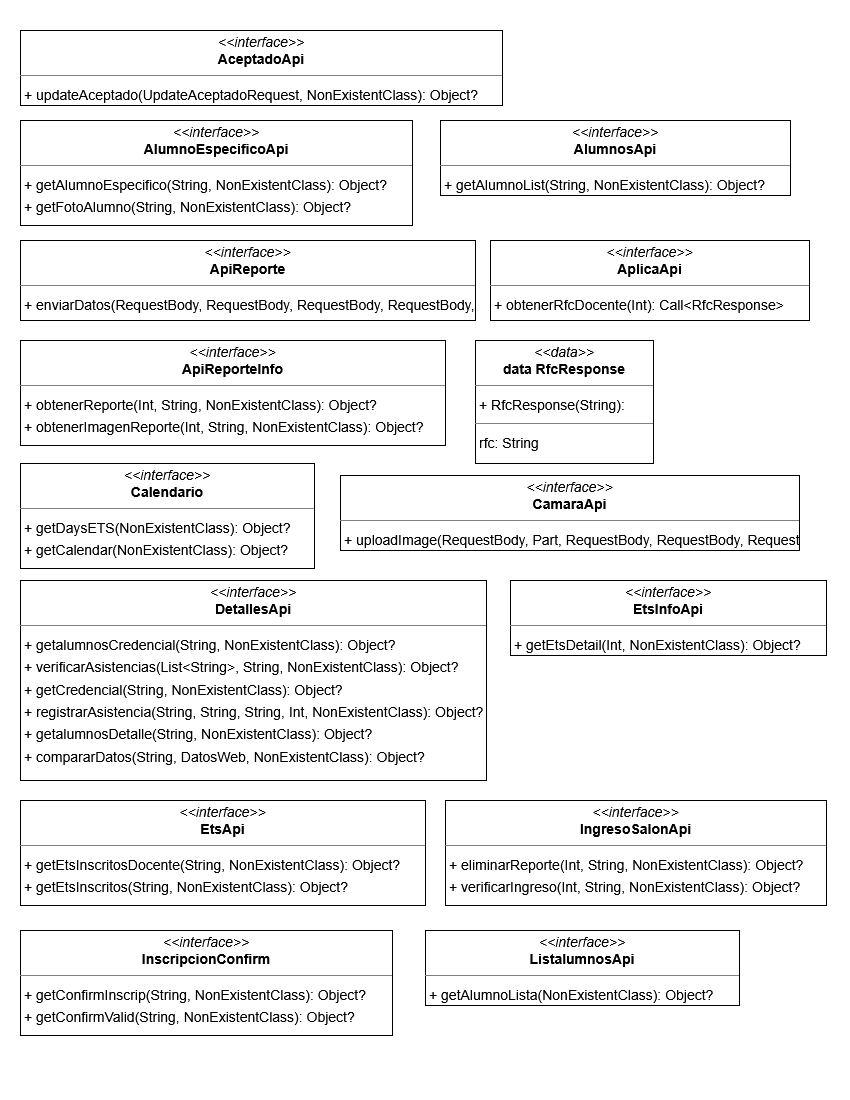
\includegraphics[width=0.75\textwidth]{DiagramasMoviles/DCM (10)}
		\caption{Diagrama de clases para package Retrofit parte 1.}
		\label{fig:Retrofit1}
	\end{center}
\end{figure}

\newpage

\subsection{Diagrama de clases de package Retrofit parte 2}

La Figura \ref{fig:Retrofit2} muestra la segunda parte del diagrama de clases de package Retrofit.

\begin{figure}[htbp!]
	\begin{center}
		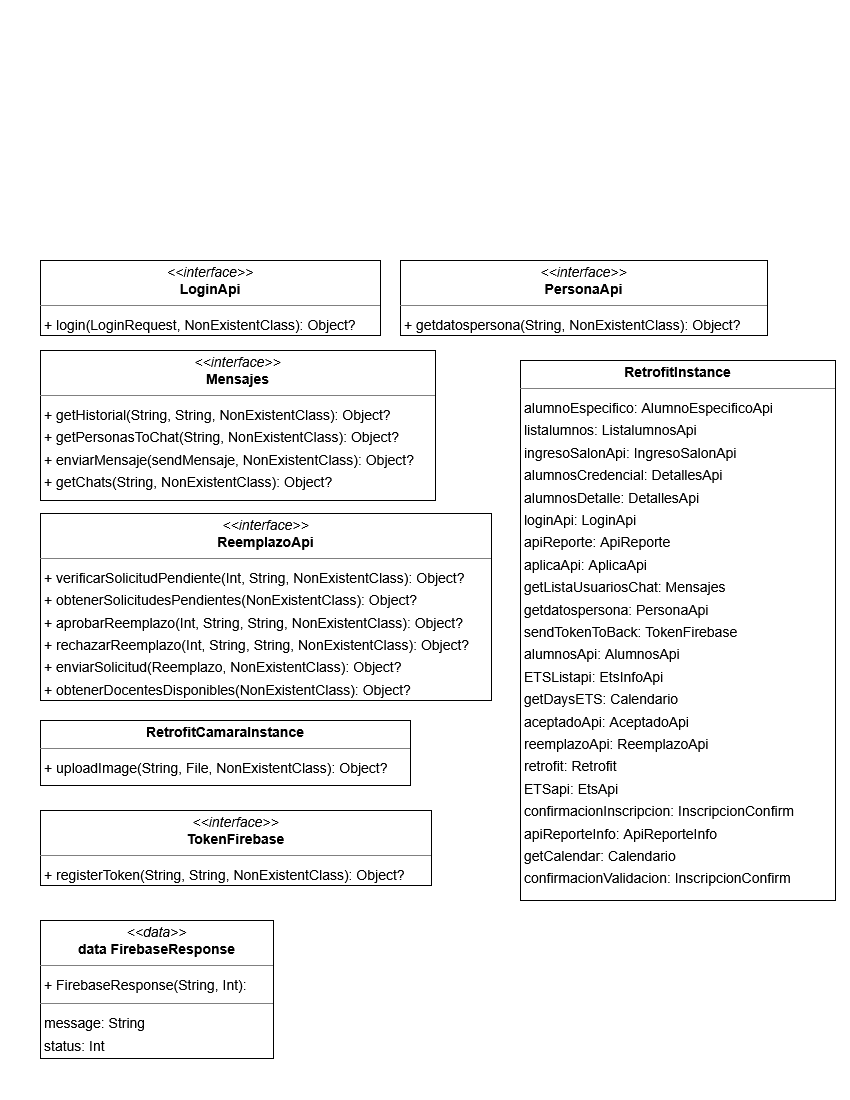
\includegraphics[width=0.75\textwidth]{DiagramasMoviles/DCM (11)}
		\caption{Diagrama de clases para package Retrofit parte 2.}
		\label{fig:Retrofit2}
	\end{center}
\end{figure}

\newpage

\section{Clases de com.example.prueba3.Clases}

Esta sección se dedica a la presentación de las Clases que constituyen el modelo de datos de la aplicación, ubicadas principalmente en el paquete `com.example.prueba3.Clases`. Como se indicó en la Figura \ref{fig:Diagrama_app_movil_detallado} (en la sección de Estructura Interna Detallada de la Aplicación Móvil), estas clases son fundamentales para la manipulación y el transporte de información dentro de la aplicación.

La mayoría de estas clases son Data Classes, un tipo de clase concisa en Kotlin diseñada específicamente para contener datos. Su función principal es servir como contenedores de información, estructurando los datos que se obtienen de los servicios remotos (a través de `RetroFit`), los que se manipulan dentro de la lógica de negocio, y los que finalmente se presentan en la interfaz de usuario a través de los `Views` (ViewModels). Estas clases aseguran la consistencia y la tipificación estricta de los datos a lo largo de todo el flujo de la aplicación.

A continuación, se mostrarán las imágenes de las Data Classes que conforman el paquete llamado `com.example.prueba3.Clases`. Cada imagen representará la estructura de una clase de datos, incluyendo sus propiedades (atributos) y tipos de datos, proporcionando una visión clara de cómo se modela la información esencial que fluye entre los componentes de la aplicación.

\newpage

\subsection{Diagrama de clases de com.example.prueba3.Clases parte 1}

La Figura \ref{fig:Clases1} muestra la primera parte del diagrama de clases de com.example.prueba3.Clases.

\begin{figure}[htbp!]
	\begin{center}
		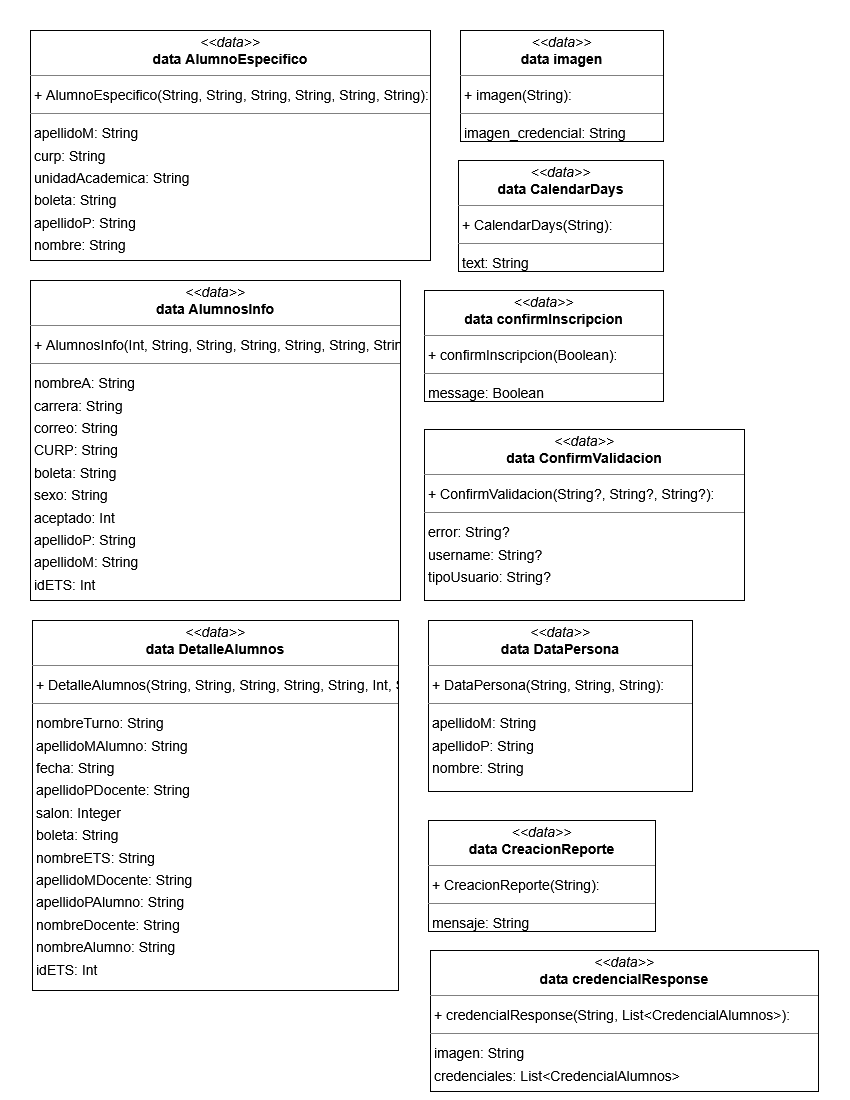
\includegraphics[width=0.75\textwidth]{DiagramasMoviles/DCM (2)}
		\caption{Diagrama de clases para com.example.prueba3.Clases parte 1.}
		\label{fig:Clases1}
	\end{center}
\end{figure}

\newpage

\subsection{Diagrama de clases de com.example.prueba3.Clases parte 2}

La Figura \ref{fig:Clases2} muestra la segunda parte del diagrama de clases de com.example.prueba3.Clases.

\begin{figure}[htbp!]
	\begin{center}
		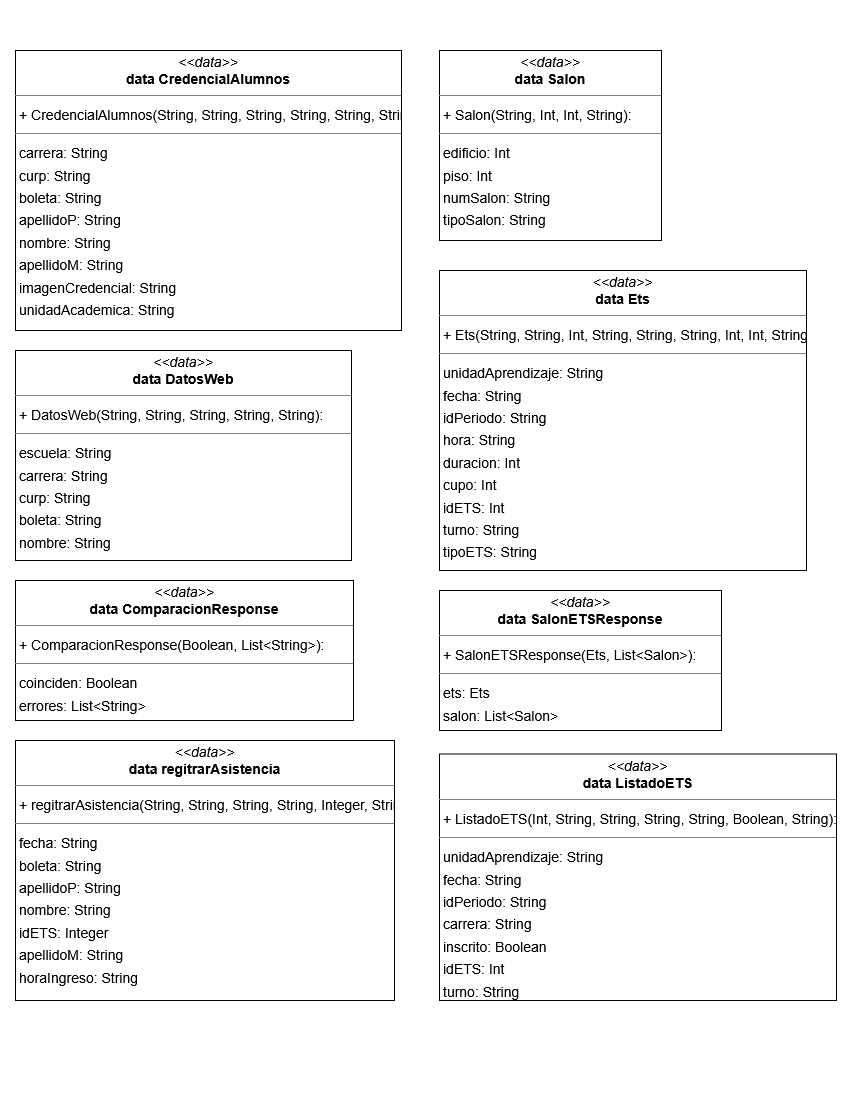
\includegraphics[width=0.75\textwidth]{DiagramasMoviles/DCM (3)}
		\caption{Diagrama de clases para com.example.prueba3.Clases parte 2.}
		\label{fig:Clases2}
	\end{center}
\end{figure}

\newpage

\subsection{Diagrama de clases de com.example.prueba3.Clases parte 3}

La Figura \ref{fig:Clases3} muestra la tercera parte del diagrama de clases de com.example.prueba3.Clases.

\begin{figure}[htbp!]
	\begin{center}
		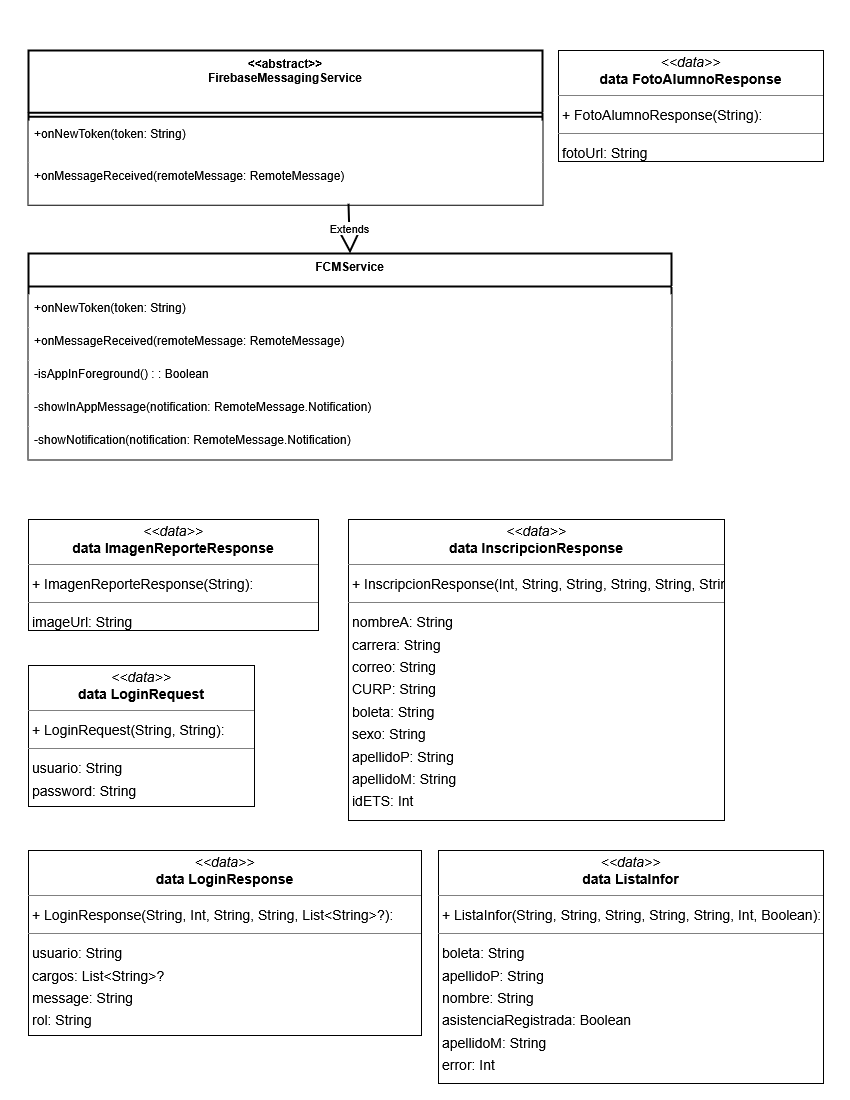
\includegraphics[width=0.75\textwidth]{DiagramasMoviles/DCM (4)}
		\caption{Diagrama de clases para com.example.prueba3.Clases parte 3.}
		\label{fig:Clases3}
	\end{center}
\end{figure}

\newpage

\subsection{Diagrama de clases de com.example.prueba3.Clases parte 4}

La Figura \ref{fig:Clases4} muestra la cuarta parte del diagrama de clases de com.example.prueba3.Clases.

\begin{figure}[htbp!]
	\begin{center}
		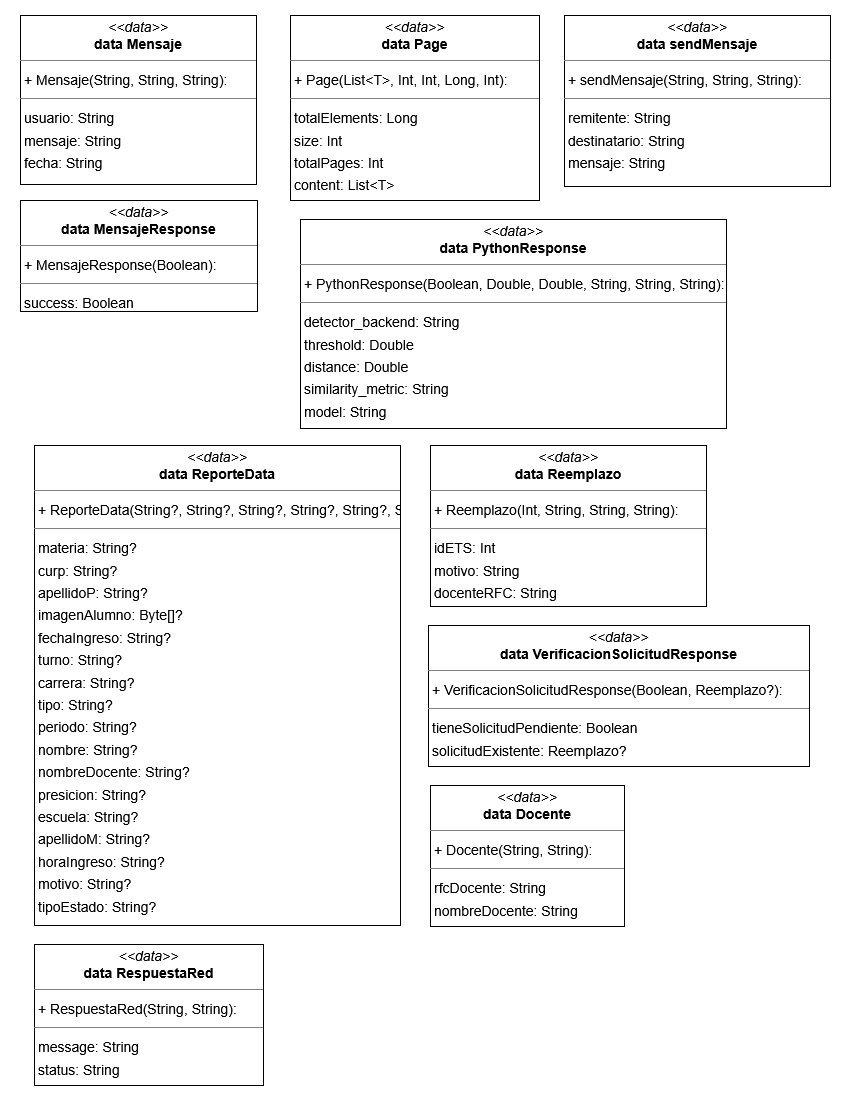
\includegraphics[width=0.75\textwidth]{DiagramasMoviles/DCM (5)}
		\caption{Diagrama de clases para com.example.prueba3.Clases parte 4.}
		\label{fig:Clases4}
	\end{center}
\end{figure}

\newpage

\subsection{Diagrama de clases de com.example.prueba3.Clases parte 5}

La Figura \ref{fig:Clases5} muestra la quinta parte del diagrama de clases de com.example.prueba3.Clases.

\begin{figure}[htbp!]
	\begin{center}
		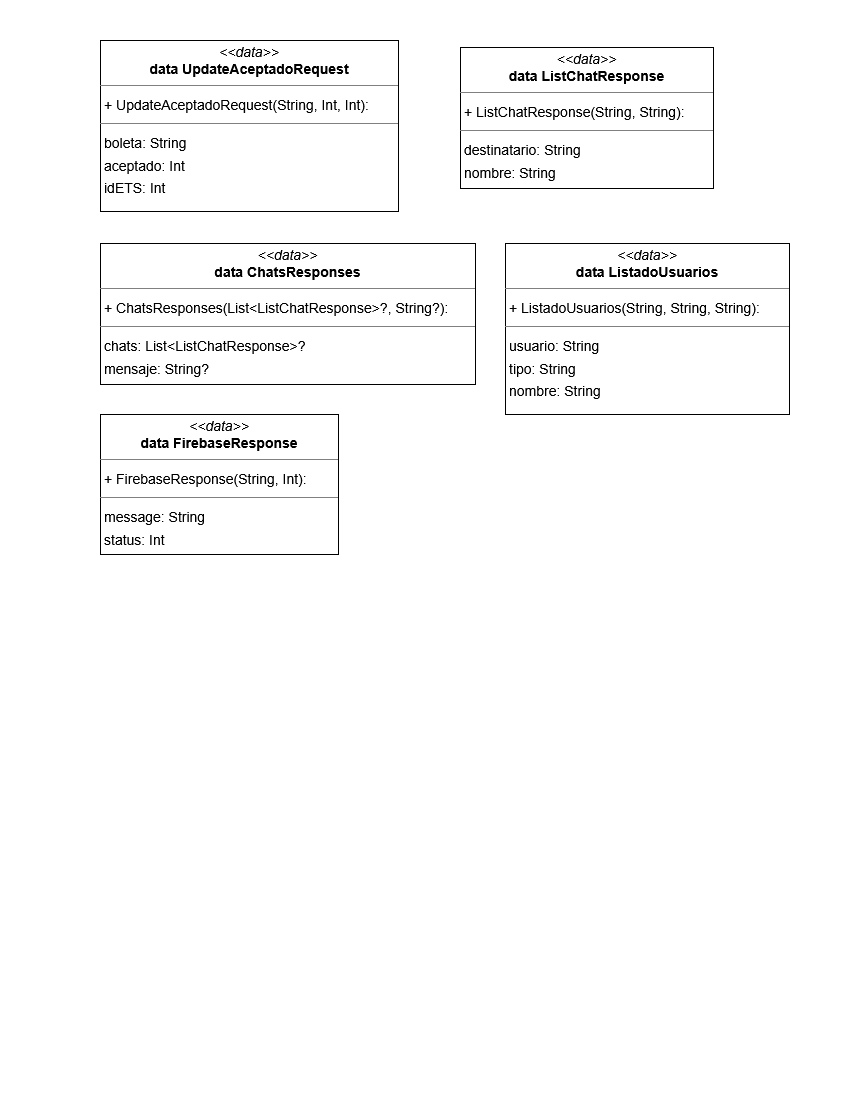
\includegraphics[width=0.75\textwidth]{DiagramasMoviles/DCM (6)}
		\caption{Diagrama de clases para com.example.prueba3.Clases parte 5.}
		\label{fig:Clases5}
	\end{center}
\end{figure}

\newpage

%\section{Diagrama de clases}

%En la figura \ref{fig:Diagrama de clases} se muestra el diagrama de clases del sistema, en el cual se establecen las clases que tenemos contempladas para ser implementadas en la creación del sistema, a su vez en este se muestran las relaciones entre las clases, los atributos que estes clases contienen y los procesos que llevaran a cabo.


%\begin{figure}[htbp!]
%	\begin{center}
%		\includegraphics[width=1\textwidth]{Clases/Clases2}
%		\caption{Diagrama de clases.}
%		\label{fig:Diagrama de clases}
%	\end{center}
%\end{figure}


\section{Diagramas de secuencia}

A continuación, se presentan los diagramas de secuencia identificados para para la propuesta de solución presentada en este documento.
En ellos se busca ilustrar el funcionamiento dinamico del sistema y modelar las interacciones entre los distintos componentes y actores dependiendo de los casos de uso descritos en el capitulo 4. 
Cada diagrama representa el flujo de mensajes e información entre los actores y las capas de la aplicación en función de la arquitectura de una aplicación basada en Spring boot.

\subsection{SE-01 Iniciar sesión del sistema móvil}

\begin{figure}[htbp!]
	\begin{center}
		\fbox{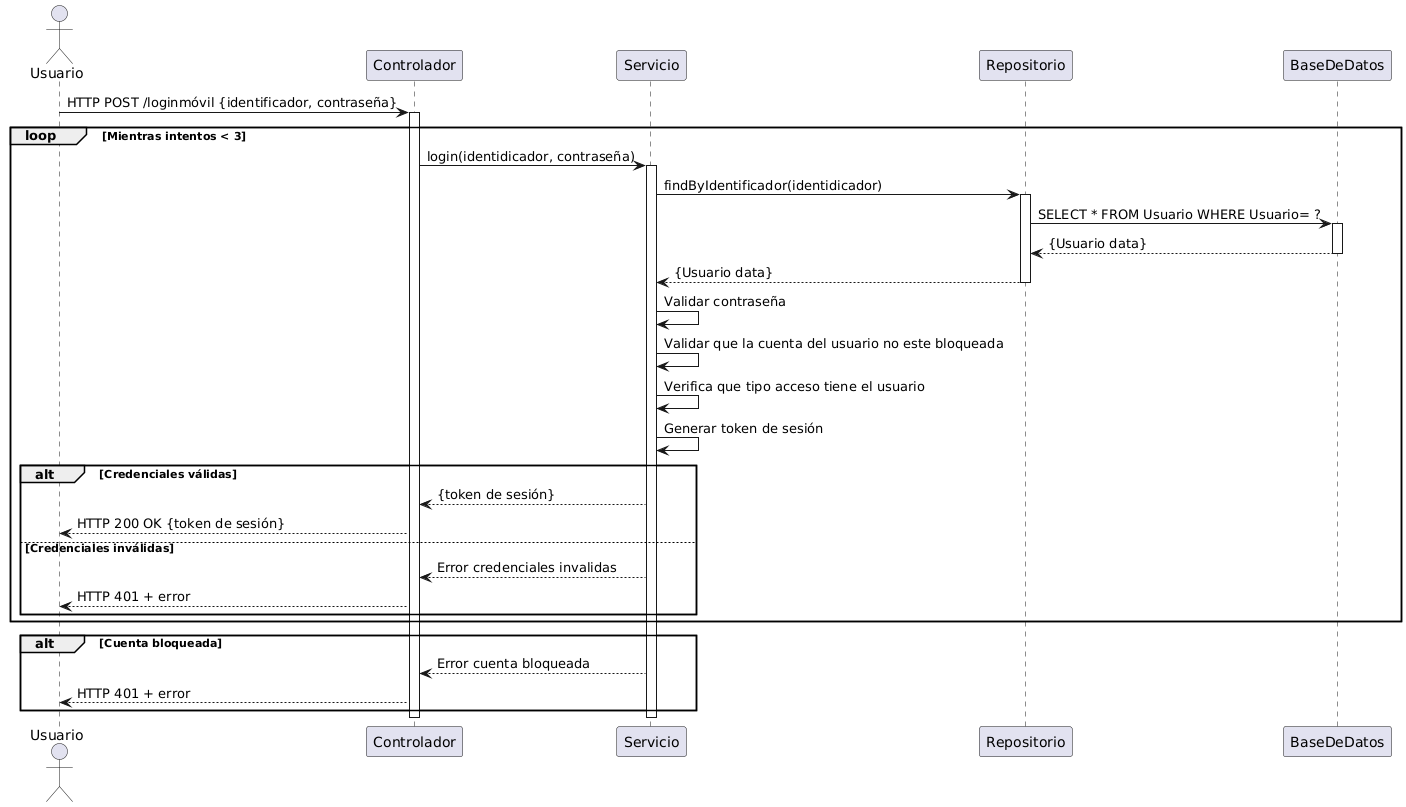
\includegraphics[width=1\textwidth]{Secuencia/CU-01.png}}
		\caption{Diagrama de secuencia del caso de uso número 01 (Iniciar sesión del sistema móvil).}
		\label{fig:Diagrama de secuencia CU-01}
	\end{center}
\end{figure}

En el diagrama de secuencia \ref{fig:Diagrama de secuencia CU-01} de secuencia se describe el proceso planeado para el caso de uso \hyperlink{CU-01}{CU-01 Iniciar sesión del sistema móvil}, mostrando las interacciones que tendrá con la vista, el controlador, el servicio, el repositorio y la base de datos.

\newpage

\subsection{SE-02 Consultar calendario escolar}

\begin{figure}[htbp!]
	\begin{center}
		\fbox{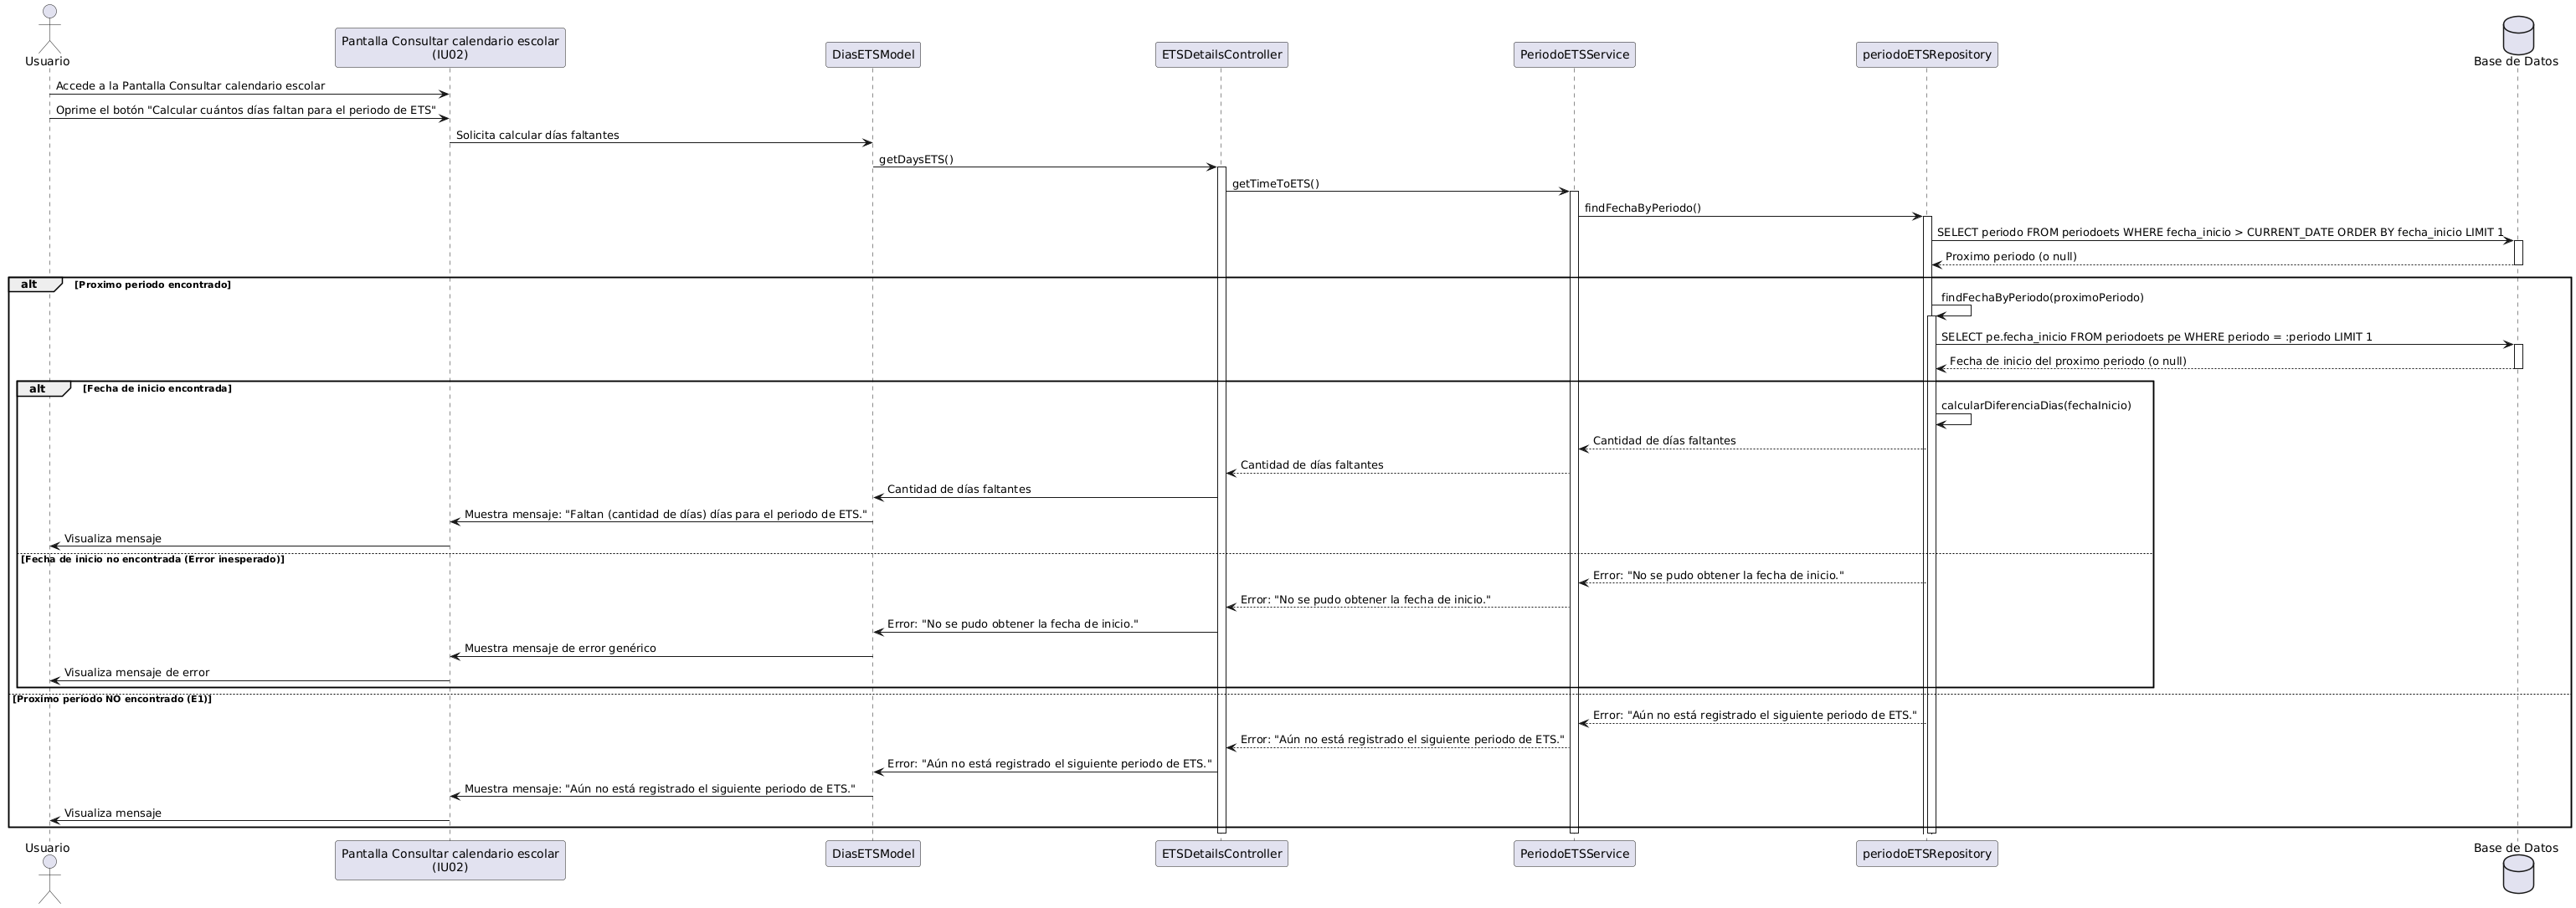
\includegraphics[width=1\textwidth]{Secuencia/CU-02.png}}
		\caption{Diagrama de secuencia del caso de uso número 02 (Consultar calendario escolar).}
		\label{fig:Diagrama de secuencia CU-02}
	\end{center}
\end{figure}

En el diagrama de secuencia \ref{fig:Diagrama de secuencia CU-02} se describe el proceso planeado para el caso de uso \hyperlink{CU-02}{CU-02 Consultar calendario escolar}, mostrando las interacciones que tendrá con la vista, el controlador, el servicio, el repositorio y la base de datos.

\newpage

\subsection{SE-03 Consultar notificaciones}

\begin{figure}[htbp!]
	\begin{center}
		\fbox{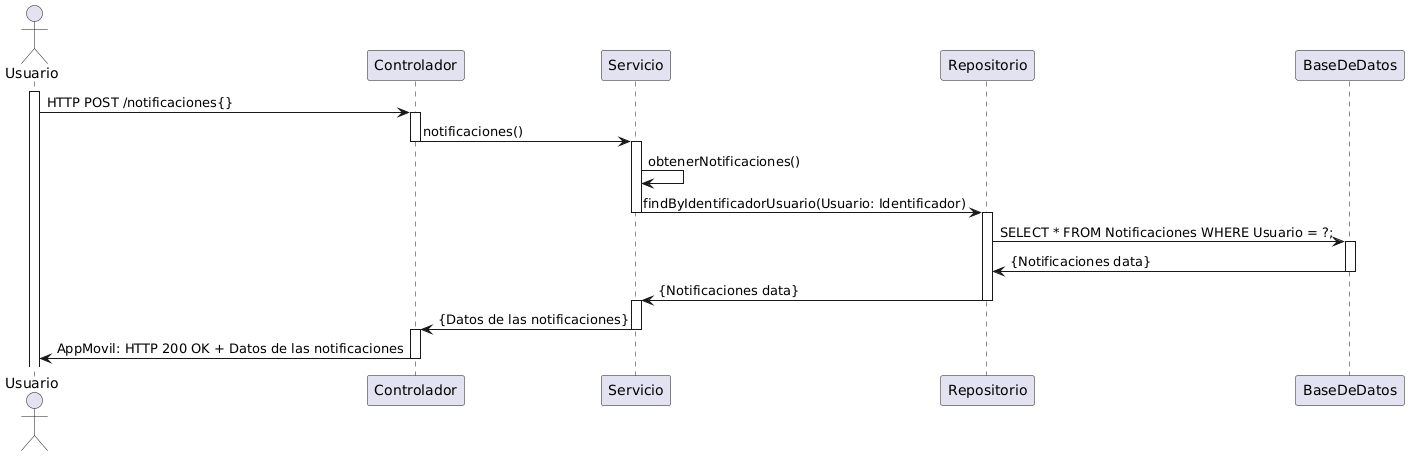
\includegraphics[width=1\textwidth]{Secuencia/CU-03.png}}
		\caption{Diagrama de secuencia del caso de uso número 03 (Consultar notificaciones).}
		\label{fig:Diagrama se secuencia CU-03}
	\end{center}
\end{figure}

En el diagrama de secuencia \ref{fig:Diagrama de secuencia CU-03} se describe el proceso planeado para el caso de uso \hyperlink{CU-03}{CU-03 Consultar notificaciones}, mostrando las interacciones que tendrá con la vista, el controlador, el servicio, el repositorio y la base de datos.

\newpage

\subsection{SE-04 Consultar periodos de ETS asignados al docente}

\begin{figure}[htbp!]
	\begin{center}
		\fbox{\includegraphics[width=1\textwidth]{Secuencia/CU-04.png}}
		\caption{Diagrama de secuencia del caso de uso número 04 (Consultar periodos de ETS asignados al docente).}
		\label{fig:Diagrama de secuencia CU-04}
	\end{center}
\end{figure}

En el diagrama de secuencia \ref{fig:Diagrama de secuencia CU-04} se describe el proceso planeado para el caso de uso \hyperlink{CU-04}{CU-04 Consultar periodos de ETS asignados al docente}, mostrando las interacciones que tendrá con la vista, el controlador, el servicio, el repositorio y la base de datos.

\newpage

\subsection{SE-05 Consultar ETS asignados}

\begin{figure}[htbp!]
	\begin{center}
		\fbox{\includegraphics[width=1\textwidth]{Secuencia/CU-05.png}}
		\caption{Diagrama de secuencia del caso de uso número 05 (Consultar ETS asignados).}
		\label{fig:Diagrama de secuencia CU-05}
	\end{center}
\end{figure}

En el diagrama de secuencia \ref{fig:Diagrama de secuencia CU-05} se describe el proceso planeado para el caso de uso \hyperlink{CU-05}{CU-05 Consultar ETS asignados}, mostrando las interacciones que tendrá con la vista, el controlador, el servicio, el repositorio y la base de datos.

\newpage

\subsection{SE-06 Mostrar información de los ETS asignados}

\begin{figure}[htbp!]
	\begin{center}
		\fbox{\includegraphics[width=1\textwidth]{Secuencia/CU-06.png}}
		\caption{Diagrama de secuencia del caso de uso número 06 (Mostrar información de los ETS asignados).}
		\label{fig:Diagrama de secuencia CU-06}
	\end{center}
\end{figure}

En el diagrama de secuencia \ref{fig:Diagrama de secuencia CU-06} se describe el proceso planeado para el caso de uso \hyperlink{CU-06}{CU-06 Mostrar información de los ETS asignados}, mostrando las interacciones que tendrá con la vista, el controlador, el servicio, el repositorio y la base de datos.

\newpage

\subsection{SE-07 Solicitar remplazo}

\begin{figure}[htbp!]
	\begin{center}
		\fbox{\includegraphics[width=1\textwidth]{Secuencia/CU-07.png}}
		\caption{Diagrama de secuencia del caso de uso número 07 (Solicitar remplazo).}
		\label{fig:Diagrama de secuencia CU-07}
	\end{center}
\end{figure}

En el diagrama de secuencia \ref{fig:Diagrama de secuencia CU-07} se describe el proceso planeado para el caso de uso \hyperlink{CU-07}{CU-07 Solicitar remplazo}, mostrando las interacciones que tendrá con la vista, el controlador, el servicio, el repositorio y la base de datos.

\newpage

\subsection{SE-08 Consultar lista de alumnos inscritos a un ETS}

\begin{figure}[htbp!]
	\begin{center}
		\fbox{\includegraphics[width=1\textwidth]{Secuencia/CU-08.png}}
		\caption{Diagrama de secuencia del caso de uso número 08 (Consultar lista de alumnos inscritos a un ETS).}
		\label{fig:Diagrama de secuencia CU-08}
	\end{center}
\end{figure}

En el diagrama de secuencia \ref{fig:Diagrama de secuencia CU-08} se describe el proceso planeado para el caso de uso \hyperlink{CU-08}{CU-08 Consultar lista de alumnos inscritos a un ETS}, mostrando las interacciones que tendrá con la vista, el controlador, el servicio, el repositorio y la base de datos.

\newpage

\subsection{SE-09 Tomar asistencias a los ETS}

\begin{figure}[htbp!]
	\begin{center}
		\fbox{\includegraphics[width=.7\textwidth]{Secuencia/CU-09.png}}
		\caption{Diagrama de secuencia del caso de uso número 09 (Tomar asistencias a los ETS).}
		\label{fig:Diagrama de secuencia CU-09}
	\end{center}
\end{figure}

En el diagrama de secuencia \ref{fig:Diagrama de secuencia CU-09} se describe el proceso planeado para el caso de uso \hyperlink{CU-09}{CU-09 Tomar asistencias a los ETS}, mostrando las interacciones que tendrá con la vista, el controlador, el servicio, el repositorio y la base de datos.

\newpage

\subsection{SE-10 Consultar lista de asistencia de alumnos inscritos a los ETS}

\begin{figure}[htbp!]
	\begin{center}
		\fbox{\includegraphics[width=1\textwidth]{Secuencia/CU-10.png}}
		\caption{Diagrama de secuencia del caso de uso número 10 (Consultar lista de asistencia de alumnos inscritos a los ETS).}
		\label{fig:Diagrama de secuencia CU-10}
	\end{center}
\end{figure}

En el diagrama de secuencia \ref{fig:Diagrama de secuencia CU-10} se describe el proceso planeado para el caso de uso \hyperlink{CU-10}{CU-10 Consultar lista de asistencia de alumnos inscritos a los ETS}, mostrando las interacciones que tendrá con la vista, el controlador, el servicio, el repositorio y la base de datos.

\newpage

\subsection{SE-11 Mostrar la foto e información  del alumno}

\begin{figure}[htbp!]
	\begin{center}
		\fbox{\includegraphics[width=1\textwidth]{Secuencia/CU-11.png}}
		\caption{Diagrama de secuencia del caso de uso número 11 (Mostrar la foto e información  del alumno).}
		\label{fig:Diagrama de secuencia CU-11}
	\end{center}
\end{figure}


En el diagrama de secuencia \ref{fig:Diagrama de secuencia CU-11} se describe el proceso planeado para el caso de uso \hyperlink{CU-11}{CU-11 Mostrar la foto e información  del alumno}, mostrando las interacciones que tendrá con la vista, el controlador, el servicio, el repositorio y la base de datos.

\newpage

\subsection{SE-12 Consultar alumno mediante código QR de la credencial}

\begin{figure}[htbp!]
	\begin{center}
		\fbox{\includegraphics[width=1\textwidth]{Secuencia/CU-12.png}}
		\caption{Diagrama de secuencia del caso de uso número 12 (Consultar alumno mediante código QR de la credencial).}
		\label{fig:Diagrama de secuencia CU-12}
	\end{center}
\end{figure}

En el diagrama de secuencia \ref{fig:Diagrama de secuencia CU-12} se describe el proceso planeado para el caso de uso \hyperlink{CU-12}{CU-12 Consultar alumno mediante código QR de la credencial}, mostrando las interacciones que tendrá con la vista, el controlador, el servicio, el repositorio y la base de datos.

\newpage

\subsection{SE-13 Buscar alumno por boleta}

\begin{figure}[htbp!]
	\begin{center}
		\fbox{\includegraphics[width=1\textwidth]{Secuencia/CU-13.png}}
		\caption{Diagrama de secuencia del caso de uso número 13 (Buscar alumno por boleta).}
		\label{fig:Diagrama de secuencia CU-13}
	\end{center}
\end{figure}

En el diagrama de secuencia \ref{fig:Diagrama de secuencia CU-13} se describe el proceso planeado para el caso de uso \hyperlink{CU-13}{CU-13 Buscar alumno por boleta}, mostrando las interacciones que tendrá con la vista, el controlador, el servicio, el repositorio y la base de datos.

\newpage

\subsection{SE-14 Buscar alumno por nombre}

\begin{figure}[htbp!]
	\begin{center}
		\fbox{\includegraphics[width=1\textwidth]{Secuencia/CU-14.png}}
		\caption{Diagrama de secuencia del caso de uso número 14 (Buscar alumno por nombre).}
		\label{fig:Diagrama de secuencia CU-14}
	\end{center}
\end{figure}

En el diagrama de secuencia \ref{fig:Diagrama de secuencia CU-14} se describe el proceso planeado para el caso de uso \hyperlink{CU-14}{CU-14 Buscar alumno por nombre}, mostrando las interacciones que tendrá con la vista, el controlador, el servicio, el repositorio y la base de datos.

\newpage

\subsection{SE-15 Registrar asistencia}

\begin{figure}[htbp!]
	\begin{center}
		\fbox{\includegraphics[width=.7\textwidth]{Secuencia/CU-15.png}}
		\caption{Diagrama de secuencia del caso de uso número 15 (Registrar asistencia).}
		\label{fig:Diagrama de secuencia CU-15}
	\end{center}
\end{figure}

En el diagrama de secuencia \ref{fig:Diagrama de secuencia CU-15} se describe el proceso planeado para el caso de uso \hyperlink{CU-15}{CU-15 Registrar asistencia}, mostrando las interacciones que tendrá con la vista, el controlador, el servicio, el repositorio y la base de datos.

\newpage

\subsection{SE-16 Consultar periodos de ETS inscritos del alumno}

\begin{figure}[htbp!]
	\begin{center}
		\fbox{\includegraphics[width=1\textwidth]{Secuencia/CU-16.png}}
		\caption{Diagrama de secuencia del caso de uso número 16 (Consultar periodos de ETS inscritos del alumno).}
		\label{fig:Diagrama de secuencia CU-16}
	\end{center}
\end{figure}

En el diagrama de secuencia \ref{fig:Diagrama de secuencia CU-16} se describe el proceso planeado para el caso de uso \hyperlink{CU-16}{CU-16 Consultar periodos de ETS inscritos del alumno}, mostrando las interacciones que tendrá con la vista, el controlador, el servicio, el repositorio y la base de datos.

\newpage

\subsection{SE-17 Consultar ETS inscritos}

\begin{figure}[htbp!]
	\begin{center}
		\fbox{\includegraphics[width=1\textwidth]{Secuencia/CU-17.png}}
		\caption{Diagrama de secuencia del caso de uso número 04 (Consultar ETS inscritos).}
		\label{fig:Diagrama de secuencia CU-17}
	\end{center}
\end{figure}

En el diagrama de secuencia \ref{fig:Diagrama de secuencia CU-17} se describe el proceso planeado para el caso de uso \hyperlink{CU-17}{CU-17 Consultar  ETS inscritos}, mostrando las interacciones que tendrá con la vista, el controlador, el servicio, el repositorio y la base de datos.

\newpage

\subsection{SE-18 Mostrar información del los ETS inscritos}

\begin{figure}[htbp!]
	\begin{center}
		\fbox{\includegraphics[width=1\textwidth]{Secuencia/CU-18.png}}
		\caption{Diagrama de secuencia del caso de uso número 18 (Mostrar información del los ETS inscritos).}
		\label{fig:Diagrama de secuencia CU-18}
	\end{center}
\end{figure}

En el diagrama de secuencia \ref{fig:Diagrama de secuencia CU-18} se describe el proceso planeado para el caso de uso \hyperlink{CU-18}{CU-18 Mostrar información del los ETS inscritos}, mostrando las interacciones que tendrá con la vista, el controlador, el servicio, el repositorio y la base de datos.

\newpage

\subsection{SE-19 Probar reconocimiento facial}

\begin{figure}[htbp!]
	\begin{center}
		\fbox{\includegraphics[width=1\textwidth]{Secuencia/CU-19.png}}
		\caption{Diagrama de secuencia del caso de uso número 19 (Probar reconocimiento facial).}
		\label{fig:Diagrama de secuencia CU-19}
	\end{center}
\end{figure}

En el diagrama de secuencia \ref{fig:Diagrama de secuencia CU-19} se describe el proceso planeado para el caso de uso \hyperlink{CU-19}{CU-19 Probar reconocimiento facial}, mostrando las interacciones que tendrá con la vista, el controlador, el servicio, el repositorio y la base de datos.

\newpage

\subsection{SE-20 Revisar información de acceso a los ETS}

\begin{figure}[htbp!]
	\begin{center}
		\fbox{\includegraphics[width=1\textwidth]{Secuencia/CU-20.png}}
		\caption{Diagrama de secuencia del caso de uso número 20 (Revisar información de acceso a los ETS).}
		\label{fig:Diagrama de secuencia CU-20}
	\end{center}
\end{figure}

En el diagrama de secuencia \ref{fig:Diagrama de secuencia CU-20} se describe el proceso planeado para el caso de uso \hyperlink{CU-20}{CU-20 Revisar información de acceso a los ETS}, mostrando las interacciones que tendrá con la vista, el controlador, el servicio, el repositorio y la base de datos.

\newpage

\subsection{SE-21 Dar de alta a alumno}

\begin{figure}[htbp!]
	\begin{center}
		\fbox{\includegraphics[width=1\textwidth]{Secuencia/CU-21.png}}
		\caption{Diagrama de secuencia del caso de uso número 21 (Dar de alta a alumno).}
		\label{fig:Diagrama de secuencia CU-21}
	\end{center}
\end{figure}

En el diagrama de secuencia \ref{fig:Diagrama de secuencia CU-21} se describe el proceso planeado para el caso de uso \hyperlink{CU-21}{CU-21 Dar de alta a alumno}, mostrando las interacciones que tendrá con la vista, el controlador, el servicio, el repositorio y la base de datos.

\newpage

\subsection{SE-22 Crear credencial y capturar fotografía estudiantil}

\begin{figure}[htbp!]
	\begin{center}
		\fbox{\includegraphics[width=1\textwidth]{Secuencia/CU-22_23.png}}
		\caption{Diagrama de secuencia del caso de uso número 22 y 23 (Crear credencial y capturar fotografía estudiantil).}
		\label{fig:Diagrama de secuencia CU-22 y CU23}
	\end{center}
\end{figure}

En el diagrama de secuencia \ref{fig:Diagrama de secuencia CU-22 y CU23} y se describe el proceso planeado para el caso de uso \hyperlink{CU-22}{CU-22 Crear credencia} y \hyperlink{CU-23}{CU-23 Capturar fotografía estudiantil}, mostrando las interacciones que tendrá con la vista, el controlador, el servicio, el repositorio y la base de datos.

\newpage

\subsection{SE-23 Consultar lista de periodo de ETS}

\begin{figure}[htbp!]
	\begin{center}
		\fbox{\includegraphics[width=1\textwidth]{Secuencia/CU-24.png}}
		\caption{Diagrama de secuencia del caso de uso número 24 (Consultar lista de periodo de ETS).}
		\label{fig:Diagrama de secuencia CU-24}
	\end{center}
\end{figure}

En el diagrama de secuencia \ref{fig:Diagrama de secuencia CU-24} se describe el proceso planeado para el caso de uso \hyperlink{CU-24}{CU-24 Consultar lista de periodo de ETS}, mostrando las interacciones que tendrá con la vista, el controlador, el servicio, el repositorio y la base de datos.

\newpage

\subsection{SE-24 Dar de alta de periodo de ETS}

\begin{figure}[htbp!]
	\begin{center}
		\fbox{\includegraphics[width=1\textwidth]{Secuencia/CU-25.png}}
		\caption{Diagrama de secuencia del caso de uso número 25 (Dar de alta de periodo de ETS).}
		\label{fig:Diagrama de secuencia CU-25}
	\end{center}
\end{figure}

En el diagrama de secuencia \ref{fig:Diagrama de secuencia CU-25} se describe el proceso planeado para el caso de uso \hyperlink{CU-25}{CU-25 Dar de alta de periodo de ETS}, mostrando las interacciones que tendrá con la vista, el controlador, el servicio, el repositorio y la base de datos.

\newpage

\subsection{SE-25 Consultar lista de ETS}

\begin{figure}[htbp!]
	\begin{center}
		\fbox{\includegraphics[width=1\textwidth]{Secuencia/CU-28.png}}
		\caption{Diagrama de secuencia del caso de uso número 28 (Consultar lista de ETS).}
		\label{fig:Diagrama de secuencia CU-28}
	\end{center}
\end{figure}

En el diagrama de secuencia \ref{fig:Diagrama de secuencia CU-28} se describe el proceso planeado para el caso de uso \hyperlink{CU-28}{CU-28 Consultar lista de ETS}, mostrando las interacciones que tendrá con la vista, el controlador, el servicio, el repositorio y la base de datos.

\newpage

\subsection{SE-26 Dar de alta ETS}

\begin{figure}[htbp!]
	\begin{center}
		\fbox{\includegraphics[width=1\textwidth]{Secuencia/CU-29.png}}
		\caption{Diagrama de secuencia del caso de uso número 29 (Dar de alta ETS).}
		\label{fig:Diagrama de secuencia CU-29}
	\end{center}
\end{figure}

En el diagrama de secuencia \ref{fig:Diagrama de secuencia CU-29} se describe el proceso planeado para el caso de uso \hyperlink{CU-29}{CU-29 Dar de alta ETS}, mostrando las interacciones que tendrá con la vista, el controlador, el servicio, el repositorio y la base de datos.

\newpage

\subsection{SE-27 Consultar lista de personal de seguridad}

\begin{figure}[htbp!]
	\begin{center}
		\fbox{\includegraphics[width=1\textwidth]{Secuencia/CU-32.png}}
		\caption{Diagrama de secuencia del caso de uso número 32 (Consultar lista de personal de seguridad).}
		\label{fig:Diagrama de secuencia CU-32}
	\end{center}
\end{figure}

En el diagrama de secuencia \ref{fig:Diagrama de secuencia CU-32} se describe el proceso planeado para el caso de uso \hyperlink{CU-32}{CU-32 Consultar lista de personal de seguridad}, mostrando las interacciones que tendrá con la vista, el controlador, el servicio, el repositorio y la base de datos.

\newpage

\subsection{SE-28 Dar de alta personal de seguridad}

\begin{figure}[htbp!]
	\begin{center}
		\fbox{\includegraphics[width=1\textwidth]{Secuencia/CU-33.png}}
		\caption{Diagrama de secuencia del caso de uso número 33 (Dar de alta personal de seguridad).}
		\label{fig:Diagrama de secuencia CU-33}
	\end{center}
\end{figure}

En el diagrama de secuencia \ref{fig:Diagrama de secuencia CU-33} se describe el proceso planeado para el caso de uso \hyperlink{CU-33}{CU-33 Dar de alta personal de seguridad}, mostrando las interacciones que tendrá con la vista, el controlador, el servicio, el repositorio y la base de datos.

\newpage

\subsection{SE-29 Consultar lista de docentes}

\begin{figure}[htbp!]
	\begin{center}
		\fbox{\includegraphics[width=1\textwidth]{Secuencia/CU-36.png}}
		\caption{Diagrama de secuencia del caso de uso número 36 (Consultar lista de docentes).}
		\label{fig:Diagrama de secuencia CU-36}
	\end{center}
\end{figure}

En el diagrama de secuencia \ref{fig:Diagrama de secuencia CU-36} se describe el proceso planeado para el caso de uso \hyperlink{CU-36}{CU-36 Consultar lista de docentes}, mostrando las interacciones que tendrá con la vista, el controlador, el servicio, el repositorio y la base de datos.

\newpage

\subsection{SE-30 Dar de alta docente}

\begin{figure}[htbp!]
	\begin{center}
		\fbox{\includegraphics[width=1\textwidth]{Secuencia/CU-37.png}}
		\caption{Diagrama de secuencia del caso de uso número 37 (Dar de alta docente).}
		\label{fig:Diagrama de secuencia CU-37}
	\end{center}
\end{figure}

En el diagrama de secuencia \ref{fig:Diagrama de secuencia CU-37} se describe el proceso planeado para el caso de uso \hyperlink{CU-37}{CU-37 Dar de alta docente}, mostrando las interacciones que tendrá con la vista, el controlador, el servicio, el repositorio y la base de datos.

\newpage

\subsection{SE-31 Solicitar desbloqueo de cuenta}

\begin{figure}[htbp!]
	\begin{center}
		\fbox{\includegraphics[width=1\textwidth]{Secuencia/CU-40.png}}
		\caption{Diagrama de secuencia del caso de uso número 40 (Solicitar desbloqueo de cuenta).}
		\label{fig:Diagrama de secuencia CU-40}
	\end{center}
\end{figure}

En el diagrama de secuencia \ref{fig:Diagrama de secuencia CU-40} se describe el proceso planeado para el caso de uso \hyperlink{CU-40}{CU-40 Solicitar desbloqueo de cuenta}, mostrando las interacciones que tendrá con la vista, el controlador, el servicio, el repositorio y la base de datos.

\newpage

\subsection{SE-32 Iniciar sesión del sistema web}

\begin{figure}[htbp!]
	\begin{center}
		\fbox{\includegraphics[width=1\textwidth]{Secuencia/CU-41.png}}
		\caption{Diagrama de secuencia del caso de uso número 41 (Iniciar sesión del sistema web).}
		\label{fig:Diagrama de secuencia CU-41}
	\end{center}
\end{figure}


En el diagrama de secuencia \ref{fig:Diagrama de secuencia CU-41} se describe el proceso planeado para el caso de uso \hyperlink{CU-41}{CU-41 Iniciar sesión del sistema web}, mostrando las interacciones que tendrá con la vista, el controlador, el servicio, el repositorio y la base de datos.

\newpage

\subsection{SE-33 Asignar docente de remplazo}

\begin{figure}[htbp!]
	\begin{center}
		\fbox{\includegraphics[width=1\textwidth]{Secuencia/CU-42.png}}
		\caption{Diagrama de secuencia del caso de uso número 42 (Asignar docente de remplazo).}
		\label{fig:Diagrama de secuencia CU-42}
	\end{center}
\end{figure}

En el diagrama de secuencia \ref{fig:Diagrama de secuencia CU-42} se describe el proceso planeado para el caso de uso \hyperlink{CU-42}{CU-42 Asignar docente de remplazo}, mostrando las interacciones que tendrá con la vista, el controlador, el servicio, el repositorio y la base de datos.